%#BIBTEX /usr/texbin/bibtex main
\documentclass[10pt,twocolumn,letterpaper]{article}

\usepackage{iccv}
\usepackage{times}
\usepackage{epsfig}
\usepackage{graphicx}
\usepackage{amsmath}
\usepackage{nccmath}
\usepackage{amssymb}
\usepackage{algorithm}
\usepackage{algorithmic}
\usepackage{tabularx}
\usepackage{comment}
%\usepackage{algpseudocode}



\newcommand{\Tref}[1]{Table~\ref{#1}}
\newcommand{\Eref}[1]{Eq.~(\ref{#1})}
\newcommand{\Fref}[1]{Fig.~\ref{#1}}
\newcommand{\Sref}[1]{Section~\ref{#1}}
\newcommand{\Aref}[1]{Algorithm~\ref{#1}}
\newcommand{\argmax}{\mathop{\rm arg~max}\limits}
\newcommand{\argmin}{\mathop{\rm arg~min}\limits}

\newcommand{\mysubsubsection}[1]{\vspace{0.1cm} \noindent \underline{{\bf #1}}:}
\newcommand{\mysubsubsubsection}[1]{\vspace{0.1cm} \noindent {\bf #1}:}
%\newcommand{\ikehata}[1]{\textcolor{blue}{ikehata:{#1}}}
%\newcommand{\yasu}[1]{\textcolor{magenta}{[yasu: {#1}]}}
%\newcommand{\hang}[1]{\textcolor{cyan}{[hang: {#1}]}}
\newcommand{\ikehata}[1]{}
\newcommand{\yasu}[1]{}
\newcommand{\hang}[1]{}

% Include other packages here, before hyperref.

% If you comment hyperref and then uncomment it, you should delete
% egpaper.aux before re-running latex.  (Or just hit 'q' on the first latex
% run, let it finish, and you should be clear).
\usepackage[pagebackref=true,breaklinks=true,letterpaper=true,colorlinks,bookmarks=false]{hyperref}

 \iccvfinalcopy % *** Uncomment this line for the final submission

\def\iccvPaperID{745} % *** Enter the ICCV Paper ID here
\def\httilde{\mbox{\tt\raisebox{-.5ex}{\symbol{126}}}}

\ifx\pdfoptionalwaysusepdfpagebox\relax\else
\pdfoptionalwaysusepdfpagebox5
\fi

% Pages are numbered in submission mode, and unnumbered in camera-ready
\ificcvfinal\pagestyle{empty}\fi
\begin{document}
	
%%%%%%%%% TITLE
\title{Structured Indoor Modeling}
	
\author{Satoshi Ikehata\\
		% For a paper whose authors are all at the same institution,
	% omit the following lines up until the closing ``}''.
	% Additional authors and addresses can be added with ``\and'',
	% just like the second author.
	% To save space, use either the email address or home page, not both
	\and
	Hang Yan\\
	Washington University in St. Louis\\
	\and
	Yasutaka Furukawa\\
}
	
\maketitle
%\thispagestyle{empty}
	
	
%%%%%%%%% ABSTRACT
\begin{abstract}
This paper presents a novel 3D modeling framework that reconstructs an
indoor scene as a structured model from panorama RGBD images. A scene
geometry is represented as a graph, where nodes correspond to structural
elements such as rooms, walls, and objects. The approach devises a
structure grammar that defines how a scene graph can be manipulated. The
grammar then drives a principled new reconstruction algorithm, where the
grammar rules are sequentially applied to recover a structured model.
%The application of the grammar automatically yields a segmented and an
%annotated 3D model.
The paper also proposes a new room segmentation algorithm and a depthmap
reconstruction algorithm that are used in the framework and can enforce
architectural shape priors far beyond existing state-of-the-art.  The
structured scene representation enables a variety of novel applications,
ranging from indoor scene visualization, automated floorplan generation,
Inverse-CAD, and more.  We have tested our framework and algorithms on
six synthetic and five real datasets with qualitative and quantitative
evaluations.
 %, compared against current state-of-the-art.
 
 
% and architectural shape reconstruction algorithms, which are top-down
% and does not rely on the primitive detection. Our framework is capable
% of producing extremely compact piecewise planar and axis-aligned 3D
% model. The structured scene representation with a compact 3D model
% enables a wide range of new applications. First, we present an indoor
% scene navigation and exploration system leveraging the extracted scene
% structure. Second, our model is CAD quality and can be directly loaded
% into a CAD software and allow user interaction. Lastly, our
% representation allows one to intuitively control the complexity of the
% output mesh model far beyond existing methods, while preserving the
% manifold-ness.  We have processed six synthetic and five real datasets,
% and compared our algorithm against various baseline and state-of-the-art
% methods. \yasu{I don't like this and need to revisit after finishing intro.}


% Unlike most existing bottom-up approaches, our method is a top-down
% approach that recovers the ``structured graph'', whose nodes correspond
% to structural elements such as room, wall, and object, and edges
% correspond to hierarchical and functional relationships of them. We then
% compile a manifold mesh by producing the mesh geometry from each leaf
% node of the graph, which enables us the element-level complexity control
% (e.g., simple wall structure and complex ceiling structure) and
% different configuration of the model (e.g., remove objects).


 
% \yasu{Put the short version of the contribution summary here.}
%\yasu{mention the number of real and synthetic datasets. mention we do
%both qualitative and quantitative evaluations on both synthetic and real
%datasets. we provide a wide range of effective applications enabled by
%the structured mdoel representation. we also compare against existing
%state-of-the-art and baseline methods.}
\end{abstract}

\section{Introduction}
%The last decade has witnessed dramatic improvements in outdoor 3D
%modeling~\cite{seitz-etal-cvpr-2006,hernandez04,Furu09c,VuCVPR09}. Their
%applications range from civil
%engineering~\cite{mani_progress_monitoring} and
%archeology~\cite{archaeology_application} in academia to digital
%mapping~\cite{google-maps}, visual effects~\cite{ILM} and 3D
%printing~\cite{123DCatch} in industry.

Indoor scenes exhibit rich geometric and functional structures, which
are carefully designed to optimize the quality of our private, social
and economic activities. A fundamental task in indoor modeling is to
discover structural elements constituting an indoor scene, such as
rooms, doors, and walls, then reconstructs a structured 3D model
consisting of such elements.
%Imagine we would have a structured indoor 3D model for every single
%building.
%A government official could take city-scale indoor 3D models to assess
%compliance with building codes, accessibility codes, and energy
%efficiency levels.
The potential applications of such 3D models range from architecture,
civil engineering, digital mapping, urban geography, real estate, and
more.

Indoor scene understanding and reconstruction has been an
active research topic in computer vision.
%thanks to the development of consumer depth sensors such as Microsoft
%Kinect~\cite{kinect_fusion}.
However, existing work has focused on small-scale indoor scenes such as
a single room or a corner of a single room
%\eg, inferring a room layout and/or object
%placements
~\cite{Hoiem13,nyu_12}.  Semantic reconstruction (SR) has been active in Computer Vision and Robotics~\cite{herbst2014toward}, but their focus is again small-scale and/or on clutter-analysis. %~\cite{lee2009geometric,Hedau2009,flint2010b,fouhey2013data,silvio_indoor_13,Hoiem13,cornel_indoor_13,nyu_12,flint2011,ssfm,hane2013joint,jia20133d,jiang2013hallucinated,herbst2014toward},
Furthermore, they assign semantics to an existing geometry, as opposed
to leverage the semantics for reconstruction.
%
Building-scale indoor modeling approaches exist. However, their output
is either a pure polygon soup~\cite{eccv_museum} or a set of planar
patches~\cite{xiong2013automatic}.
%their goal is to reconstruct a pure geometry (\ie, a polygon soup).
%, which limits applications.


%In contrast, our framework seeks to
%recover architectural information for an entire building,
%where the process of segmentation, annotation, and reconstruction
%happens simultaneously.
We establish a computational framework and algorithms for reconstructing
{\it structured indoor model} from panorama RGBD images.
% that yields structured 3D representation of an indoor scene.
We introduce a novel 3D model representation ``structure graph'', whose
nodes represent structural elements such as rooms, doors, and objects,
and the edges represent their geometric relationships. ``Structure
grammar'' then defines a list of possible graph transformations. This
grammar drives a principled new reconstruction algorithm, where the
rules are sequentially applied to naturally segment, annotate, and
reconstruct architectural scenes. 

 
The framework allows one to design a different geometric representation
(\eg, mesh, depthmap, or point-cloud) and a different reconstruction
algorithm to enforce the most effective architectural prior for each
structural element. An effective choice is possible, since our approach
is top-down and the full context is given in reconstructing each
element. 


The paper also proposes new room segmentation and offset-map
reconstruction algorithms that produce high quality yet extremely compact
3D models.
%
%The key is the enforcement of the architectural shape priors, and these
%methods are capable of producing very compact 3D models far beyond
%existing methods.
Despite the flexible representation, our framework guarantees to produce
a manifold mesh, which enables a wide range of new applications. Our
framework is evaluated qualitatively and quantitatively with both the
synthetic and real data.
%Please see the supplementary video demonstrating some of the
%applications.
% We will demonstrate a novel indoor scene viewer, an Inverse-CAD
% application, and the capability to digital map, which provides
% photo-realistic views of a scene from ground to air, shows abstracted
% floorplan, and allows one to navigate and explore a scene through
% interactions at the level of the room entities. Inverse-CAD is another
% application, where our model can be directly imported to a CAD system
% for easy human post-processing. The structured model representation
% allows one to intuitively control the complexity of the output mesh, for
% example, by specifying the maximum number of polygons allowed for each
% room, wall, or an entire scene (\eg, for mobile applications).

In summary, the contributions of the paper are three-fold:
 
\mysubsubsection{Framework contribution} A principled new structured
model representation and a reconstruction framework. This framework is
general and applicable to other domains, such as outdoor architectural
scenes or man-made objects,
%(\ie, reverse engineering),
where the subjects consist of structural elements with regularities.


\mysubsubsection{Technical contribution} A room segmentation and
reconstruction algorithm that classifies room connection types, and an
offset-map reconstruction algorithm that produces extremely compact
model by enforcing both the low-entropy and the low-rank structure in
the output label space.

\mysubsubsection{System contribution} This paper is the first to 1)
produce segmented and annotated models from the level of rooms to
objects, 2) generate floorplans automatically, and 3) enable a compelling
Inverse-CAD application for indoor scenes.


%, and 4) allows direct model-complexity control at varying levels (\eg,
%specify the maximum polygon counts for each element type).


% \eg, primitive generation and fitting~\cite{eccv_museum, Mura2014} that
% produces the ``polygonal soup'' of the indoor geometry, our approach is
% top-down, where the structure graph of the indoor scene is recovered and
% then converted into the geometry (e.g., 3D meshes). Therefore, our
% structured model allows users to control the element-level complexity of
% the model by manipulating the graph rather than the geometry, which
% enables the post-manipulation of the reconstructed model \eg, on the CAD
% system, that facilitates novel applications in science, engineering and
% commerce, which would impact our activities to a great extent.



% This structured graph representation yields a globally-consistent
% manifold mesh at the scale of a building.

% Our approach exhibits several key differences. 


% In this work, we input spherical panorama RGB-D images from sparse
% viewpoints in the indoor scene rather than using dense RGB-D stream
% like~\cite{Henry2012}. The main reason is, we consider that one of the
% main applications of the indoor modeling is the {\it exploration}, and
% an augmented sphere where the panoramas are attached allows us to
% perform novel view synthesis in all directions as will be shown in this
% paper.

% The main contributions of our paper are summarized as follow,

% % \item We propose the structured indoor scene representation that encodes the complex relationship of an indoor scene elements.
% % \item We present a complete framework and algorithms that reconstruct the structured model from sparsely distributed RGB-D panorama images.
% % \item We evaluate our framework both on synthetic and real datasets
% % and present various applications using our structured indoor
% % modeling.
% \noindent{\bf Framework constribution}: Novel structured indoor scene representation and modeling framework that is generic beyond indoor scenes.

% \noindent{\bf Technical contribution}: Room segmentation and
% reconstruction algorithm and piecewise planar 2D offsetmap
% reconstruction algorithm.

% \noindent{\bf System contribution}: A wide range of key applications
% (indoor map, inverse CAD, automatic floorplan map generation,
% intuitive complexity control). The first system to automatically
% produce segmented and annotated 3D models at a large scale.


% first paper to segmented, and annotated 3D model from the scale of an
% entire scene, room, down to an object. applications

%%\yasu{need to polish.}


%\yasu{emphasize that our method is top down and does not perform primitive extraction at all, while most existing algorithms for compact 3D modeling relies on primitive generation, which is the most problematic step of these methods, and are bottom-up.}
%
%\yasu{Emphasize that rgbd panorama is standard than kinect.}
 \section{Related Work}
This paper touches many topics in diverse fields from Computer
Vision, Computer Graphics and Robotics.
% general 3D reconstruction (Computer Vision), architectural scene
% modeling (Computer Vision and Computer Graphics), image segmentation and
% recognition (Computer Vision), and submodular optimization (Machine
% Learning).x
We here limit the discussion to closely related topics.

\mysubsubsection{Small-scale indoor modeling} Indoor scene modeling has
been active in Computer Vision, where a room layout and/or object
placements are inferred from an
image~\cite{Hedau2009,fouhey2013data}, an RGBD
image~\cite{Hoiem13,cornel_indoor_13}. Data driven
approaches with 3D model databases yield CAD-quality
reconstructions~\cite{cad_matching_12,search_classify_12}. However, the
focus of these methods is so far on a clutter analysis in a small scale
such as a single room.
% , their focus
% is mainly on analysis of the room structure in a small scale rather than
% complete geometry reconstruction of multiple rooms.
%
Semantic reconstruction (SR) from an RGBD stream has been also active in
Robotics and Computer
Vision~\cite{jia20133d,herbst2014toward}. These
methods handle slightly larger scenes, but are still not at the scale of
an entire scene with multiple rooms. Also, SR merely assigns semantics
to the pre-reconstructed 3D models. Segmentation, recognition, and
reconstruction are unified into a single formulation in
\cite{hane2013joint}, but their operating range is also small, as the
entire scene is modeled as a voxel grid.

\mysubsubsection{Large-scale indoor modeling}
Recent developments in the sensor technologies enable us to capture
dense 3D points in a large scale.
%In the domain of construction and civil engineering, automated
%acquisition of semantically rich building information models (BIMs) is a
%focus of interest. They analyze building-scale LiDAR models.
However, when it comes to the construction of a real 3D model (e.g., a
mesh), existing methods only produce a set of planar patches at a room
scale~\cite{xiong2013automatic}, simple geometric
primitives for a part of a scene~\cite{mani_progress_monitoring}, a
dense mesh staright from a voxel grid~\cite{Turner2015}, an extruded
model from a floorplan~\cite{Turner2015}, or a ``polygon soup'' without
any structure or semantics~\cite{eccv_museum}.
%
%
For large scenes, room segmentation is also an important problem. The
current state-of-the-art methods solve in a top-down 2D
domain~\cite{Turner2015,Mura2014}. Room boundaries are often ambiguous in
a top-down view, and our approach explicitly classifies room connection
types with full 3D information to solve the problem.


\mysubsubsection{Architectural shape priors}
%Geometric regularities, such as planarity and orthogonality, have been
%used for man-made scenes.
Primitive detection is combined with Markov Random Field (MRF) to
reconstruct piecewise planar depthmaps~\cite{ManhattanWorldStereo}.
Detected 3D primitives can be assembled directly in the 3D
space~\cite{eccv_museum}.  However, excessive number of
primitives need to be extracted not to miss a single important one, and
the primitive detecion often becomes the most problematic step. Instead,
we combine MRF with Robust Principal Component Analysis
(RPCA)~\cite{Candes2011} to enforce both the low-entropy and the low-rank
structure in the depthmap to obtain much more compact 3D
models without relying on the primitives.

% which is exacerbated by the curse of dimensionality, where only very
% simple primitive types can be used.
%
%Primitive generation has been combined with a popular bottom-up
%formulation, Markov Random Field (MRF) for
%robustness~\cite{MRF_middlebury,MRF_evaluation_2013}.
%
%  For example, in a case of a depthmap estimation,
% one of the extracted primitives, instead of a discretized depth value,
% is assigned to each pixel

% These methods enforce geometric regularities fairly well, but the models
% are still a ``polygon soup'' without any structure or semantic
% information~\cite{ManhattanWorldStereo,GallupPlanar10,SinhaPlane09,lukas2008ffa}. They
% also lack in the ability to effectively control the model complexities.

%\mysubsubsection{Structured reconstruction} A seminal work by Dick et
%al.~\cite{Cipolla_MCMC} employs Markov Chain Monte Carlo (MCMC) to reconstruct
%structured outdoor building models. 2.5D facade
%models are reconstructed from images by following a shape
%grammar~\cite{ProceduralFacade}.
%% When it comes to building facades, which exhibit strong structural patterns,
%% 2.5D facade models are reconstructed from images by following shape
%% grammars
%The detection and parsing, although not necessarily the reconstruction,
%of outdoor buildings were demonstrated from LiDAR point clouds by
%applying a simple grammar~\cite{toshev2010detecting}. However, all these
%methods handle outdoor scenes, which are usually much simpler.
%and free from clutter.
%We have produced a recent breakthrough in indoor 3D modeling, where
%constructive solid geometry (CSG) is used to reconstruct large museum
%interior models~\cite{eccv_museum}.
% including Met museum in NYC, one of the
% largest art galleries in the world.

 \section{Structured Modeling}
%\ikehata{The titles of section 3 and section 4 are quite similar. Is
%that on purpose?}
% \begin{table*}
% 	\caption{Properties of elements in the structured indoor scene representation. }
% 	\begin{tabularx}{160mm}{|c|X|X|}
% 		\hline Element Type & Properties & Description \\
% 		\hline\hline Room ($\textbf{R}$) &  RoomId & Index of the room\\
% 		\hline  &  PixelIdList & Pixel index list\\ 
% 		\hline Wall ($\textbf{W}$)  & WallId &  Index of the wall\\ 
% 		\hline  &  pRoomId & Parent room index \\
% 		\hline  &  nWallId1 & Previous wall index \\ 
% 		\hline  &  nWallId2 & Next wall index \\ 
% 		\hline  &  PixelIdList & Pixel index list \\ 
% 		\hline  &  VoxelIdList & Voxel index list \\
% 		\hline  Wall Details ($\textbf{WD}$) & pWallId & Parent wall index \\
% 		\hline  &  VoxelIdList & Voxel index list  \\ 
% 		\hline Door ($\textbf{D}$) &  DoorId & Index of the door\\ 
% 		\hline  &  pWallId1 & Parent wall index (first)\\ 
% 		\hline  &  pWallId2 & Parent wall index (second) \\ 
% 		\hline  &  Corner1 & Door corners on the wall (first)\\ 
% 		\hline  &  Corner2 & Door corners on the wall (second) \\ 
% 		\hline Ceil, Floor ($\textbf{C}, \textbf{F}$) & CeilId, FloorId & Index of the ceil/floor \\
% 		\hline  & pRoomId & Parent room index\\ 
% 		\hline  &  Z & Height of the basis plane \\ 
% 		\hline  &  VoxelIdList & Voxel index list \\
% 		\hline  Ceil Details ($\textbf{CD}$) & pCeilId & Parent ceil index \\
% 		\hline  &  VoxelIdList & Voxel index list  \\ 
% 		\hline Object ($\textbf{O}$) & pRoomId & Parent room index\\ 
% 		\hline  &  PointIdList & Point index list \\ 
% 		\hline  
% 	\end{tabularx} 
% \end{table*}

The key innovation lies in the structured representation of scene
geometries, and its reconstruction framework. We represent a scene as a
``structure graph'' and conduct reconstruction as a
sequence of ``structure grammar'' applications. This section presents
these key concepts (See Fig.~\ref{fig:graph_grammar}).
%, where the grammar defines a set of rules to manipulate the structure
%graph (See Fig.~\ref{fig:graph_grammar}).

\begin{figure*}[tb]
% 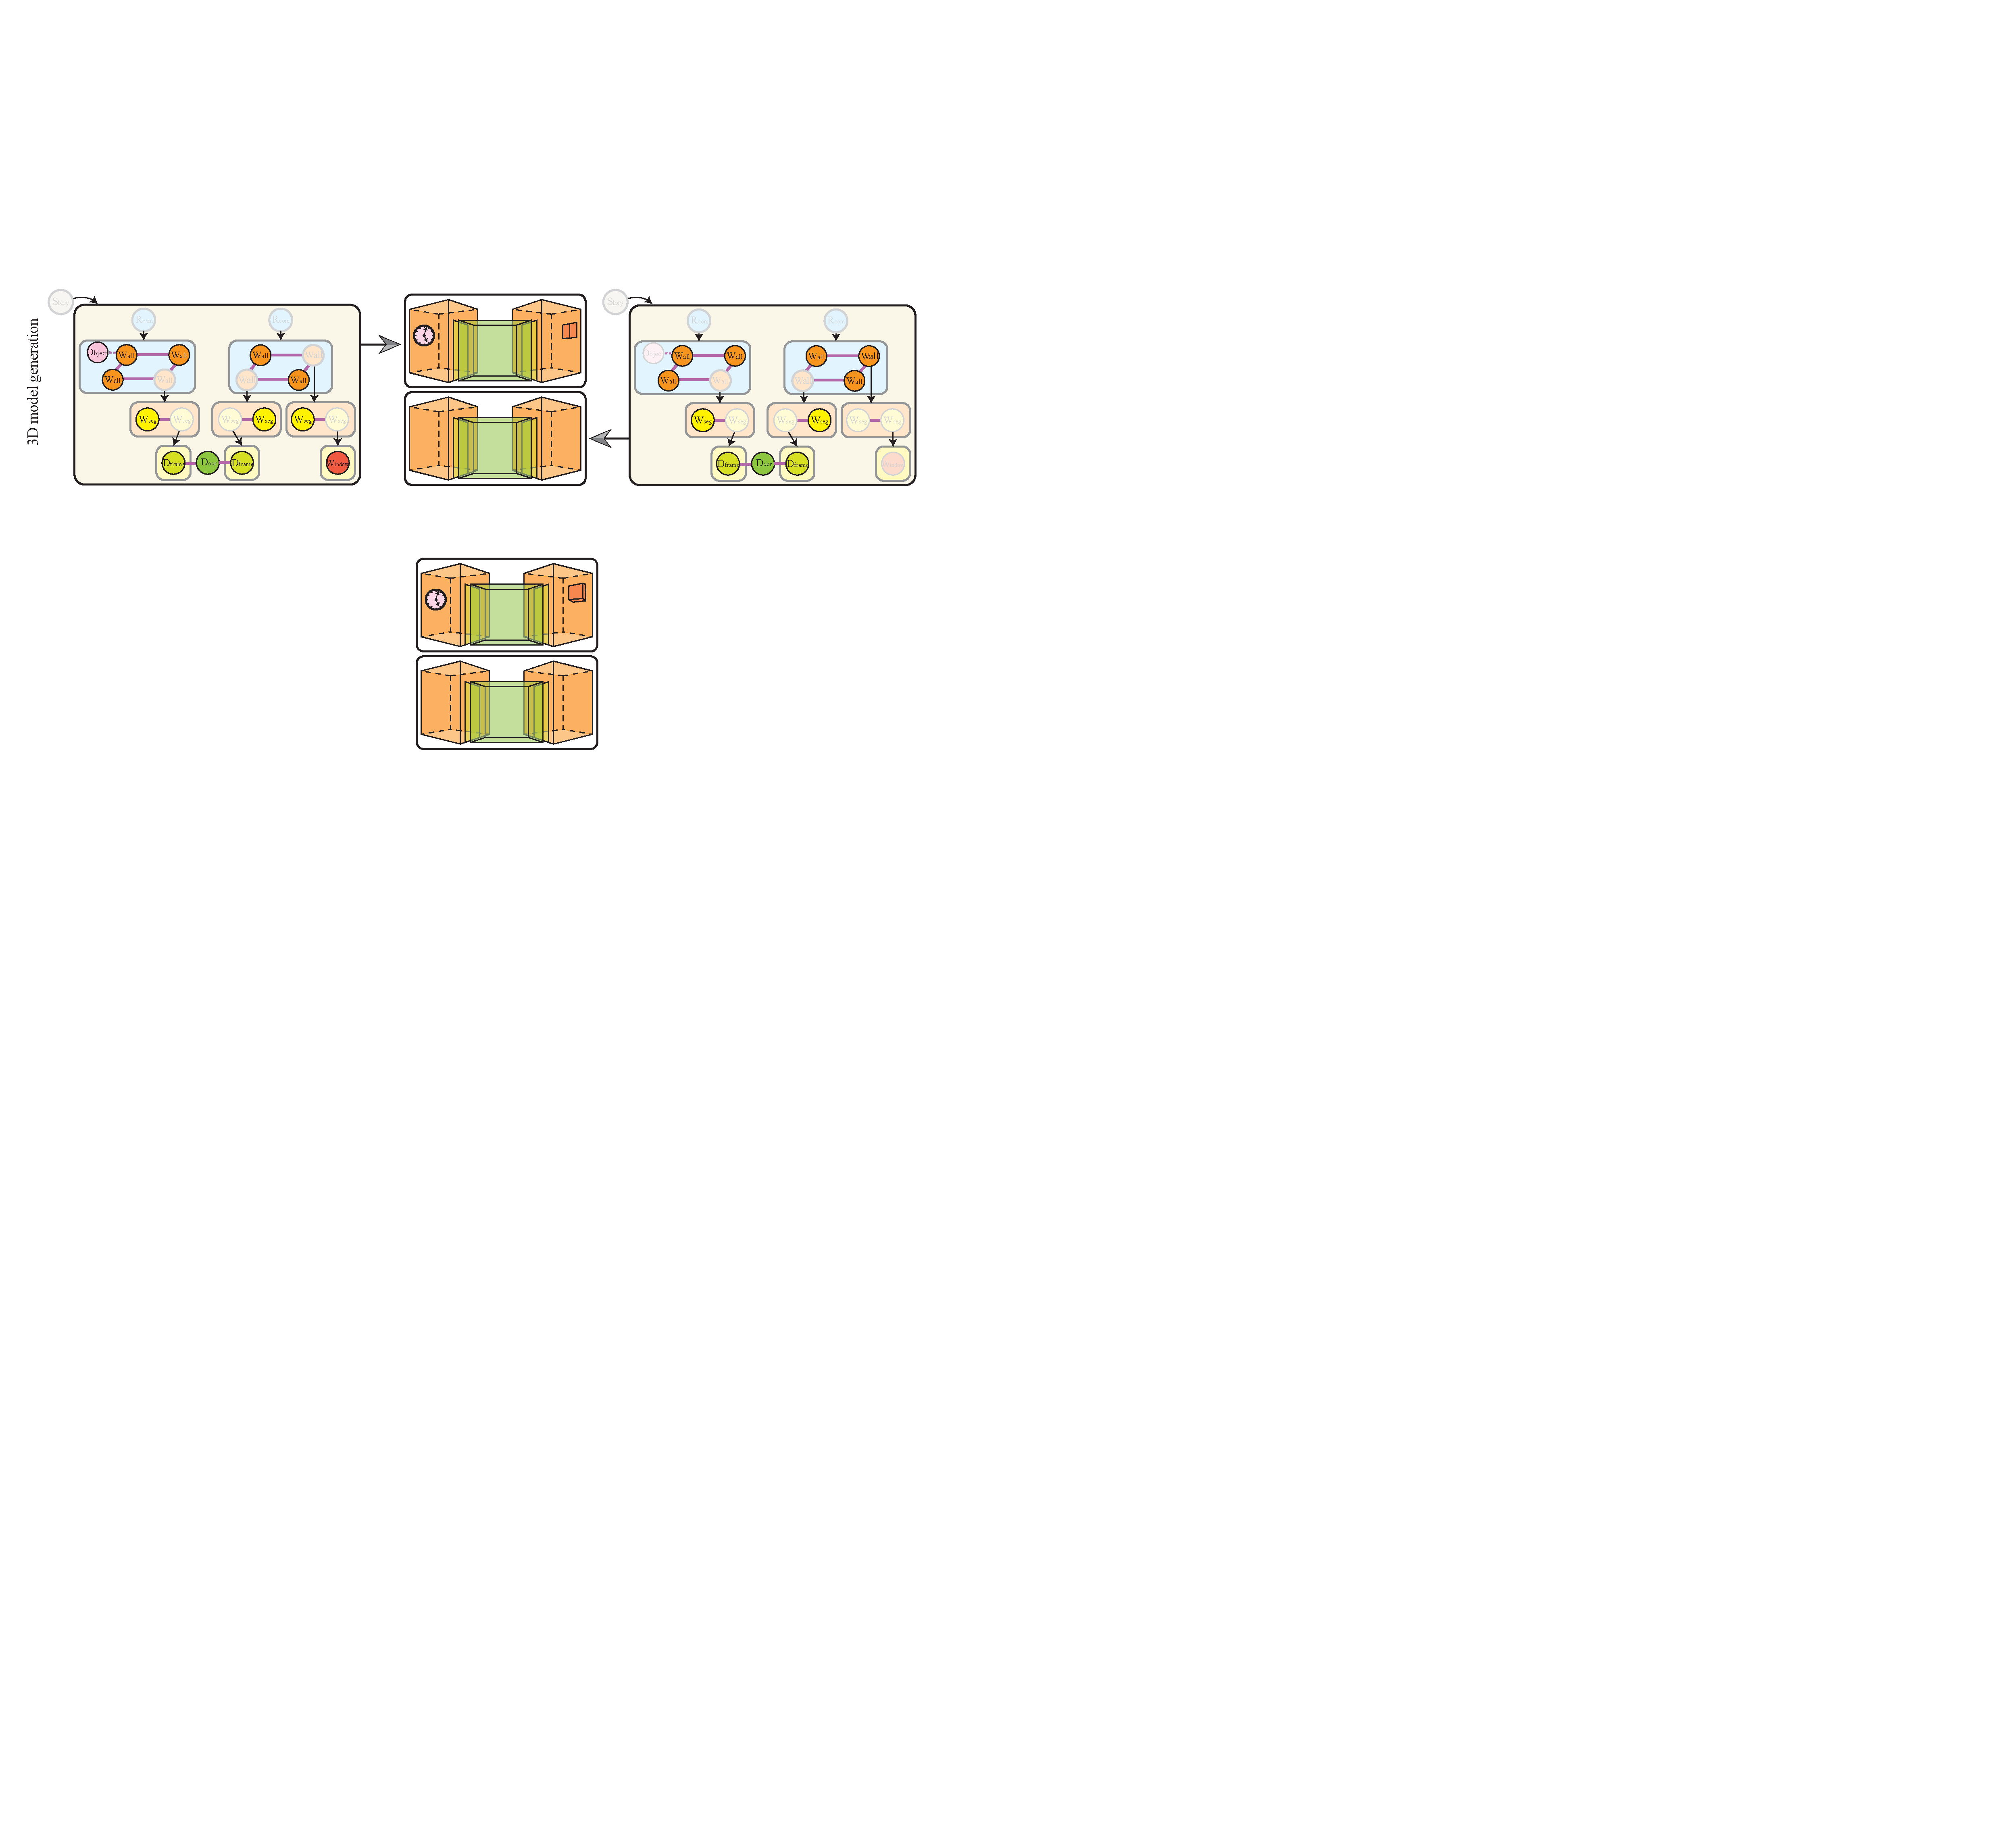
\includegraphics[width=\textwidth]{../figures/model.pdf}
\begin{center}
 \includegraphics[width=150mm]{../figures/grammar.pdf} 
 \end{center}
 \caption{Top
 left: An indoor scene is modeled as a {\em structure graph}, where
 nodes correspond to structural elements such as a room, a door, or an
 object. Each node is associated with a geometry such as a mesh or a
 depthmap, except for the scene and the room nodes. Edges contain their
 geometric relationships. A mesh model can be generated from the graph
 by outputting a mesh from every leaf node (a node without an out-going
 directed edge). Top right: One can drop an arbitrary set of nodes from
 the leaves for the mesh generation. As long as no dangling solid
 undirected edges remain, the mesh is guaranteed to be a
 manifold. Bottom: {\em Structure grammar} defines a set of possible
 transformations of this graph. Our reconstruction process is
 to sequentially apply these rules to recover the structure graph.}
 \label{fig:graph_grammar}
 \vspace{-0.325cm}
\end{figure*}

\mysubsubsection{Structure graph}
%\subsection{Structure graph}
A scene geometry is represented as a graph, where nodes correspond to
structural elements such as a room, a wall, and an object. Each node is
associated with geometry (e.g., a mesh, a depthmap, or voxels)
with the exception of ``scene'' and ``room'', which are abstract
elements. Our model works with any geometric representation, and even
allows different representations for different elements (e.g., a solid
for a room and a mesh for an object).

Nodes are connected by three types of edges.
%First, there are two types of undirected edges.
First, when structural elements have a common surface boundary (e.g.,
adjacent wall nodes), the nodes are connected by a solid undirected edge
(purple in Fig.~\ref{fig:graph_grammar}), enforcing that the geometries
match exactly along the boundary. This geometric consistency, dubbed
``boundary condition'', is the key to guarantee manifold-ness later. A
dashed undirected edge, on the other hand, represents an attachment
relationship without the boundary constraint (e.g., an object in a
room).~\footnote{We attach objects to room nodes. Give more precise
contact relationships, the framework allows one to attach to other nodes
easily (\eg, floor).}  Lastly, a directed edge encodes the
level-of-detail relationship: Structural elements at the children nodes
constitute a detailed version of the element at their parent. For
example in Fig.~\ref{fig:graph_grammar}, a ``Wall'' node contains a
simple quad surface. The child node ``Wall w/ hole''
contains a hole in the middle of the quad to represent the doorway.
% parent is a ``Wall'' node representing a simple quad surface.
Note that the boundary condition of a parent must be also satisfied by
the children nodes to guarantee the manifold-ness.

%In the above example, ``Wall'' has a boundary condition with the floor
%and the adjacent wall nodes, which must be also satisfied by the child
%node ``Wall w/ hole''.
%
% This boundary
% condition must be also satisfied by the child node ``Wall w/ hole'' so
% that the underlying scene representation exhibits a manifold regardless
% of the level of detail.
% %For example, a pair of adjacent walls are connected by this edge.


\mysubsubsection{Structure grammar}
%\subsection{Structure grammar}
Structure grammar defines a set of transformation rules that are allowed
on a structure graph, where each rule application triggers a
reconstruction algorithm. A rule has two components. 1) A
``pre-condition'' must be satisfied by the current graph to be
applicable. 2) The ``transformation'' describes how the
structure graph should change.
%
Take a room reconstruction for example. The rule takes a room node
(pre-condition). The rule produces a floor node, a ceiling node (not
shown to avoid clutter), and a chain of wall nodes (transformation).
The details of the rule set are given in Sect.~\ref{section:room}.

\mysubsubsection{Structured reconstruction}
%\subsection{Structured reconstruction}
The grammar drives our structured reconstruction process,
where the grammar rules are sequentially applied to recover a structure
graph together with the geometries. For each rule application, we choose
a geometric representation and a reconstruction algorithm that are
suitable for the task. For example, the room reconstruction rule
recovers a 1D polygon shape and extrudes it to the floor and the ceiling
heights to reconstruct a room model. The 1D polygon is obtained by a
special algorithm that is designed to produce a piecewise planar compact
polygon~\cite{Cabral2014}.
%
%This algorithm based on the dynamic programming is optimized to produce
%piecewise planar compact polygon, which is ideal to reconstruct a room
%shape.
Two types of geometric constraints need to be enforced in the
reconstruction process. First, boundary conditions must be satisfied: 1)
Existing boundary conditions (i.e., undirected solid edges) before the
rule application must be preserved; 2) New boundary conditions must be
satisfied. Second, reconstructed geometries must not intersect with the
existing geometries in the other nodes.
%The wall detail reconstruction, on the other hand, uses a 2D offset-map
%as the representation, where the combination of 2D Markov Random
%Field~\cite{label_cost_paper?} and Robust PCA~\cite{robust_pca}
%algorithms is used as the solver.
Although these constraints may appear very complex, it is fairly
straightforward to enforce them, as shown in Sect.~\ref{section:room}.

\mysubsubsection{Mesh compilation} While the structure graph is flexible
and allows different geometric representations at different nodes, it is
often desirable to produce a mesh model for applications.
%A manifold mesh enables more interesting applications as shown in
%Sect.~\ref{section:applications}.
The graph allows one to compile a manifold mesh by simply producing the
mesh geometry from each leaf node (i.e., a node without an out-going
directed edge). In the top left of Fig.~\ref{fig:graph_grammar},
non-leaf nodes are grayed-out. Here, the geometry at each node needs to
be converted to a mesh if necessary, which is easy for standard
geometric representations (e.g., a depthmap by simple meshing, a
volumetric scalar field by the Marching-Cube method~\cite{MarchingCube},
or a point cloud by Poisson Surface
Reconstruction~\cite{shan2014occluding}). Furthermore,
complexity and details of the mesh model can be easily controlled by dropping an arbitrary set of nodes from the
leaves. Since the boundary constraint at any node is satisfied by the
children, we can inductively prove that the compiled mesh model would
also be a manifold, as long as no dangling solid undirected edges
remain. Please see the supplementary material for a proof.


\mysubsubsection{Assumptions}
We assume that a scene has a single story and room structures (i.e., floor, ceiling, and walls) are aligned with the Manhattan directions. However, this is due to our particular choice of a structure grammar and reconstruction algorithms. One can certainly change the grammar and algorithms to extend the capabilities (e.g., multi-story buildings and non-Manhattan structures).
%\begin{figure}[!t]
%\begin{center}
%\includegraphics[width=85mm]{../figures/complexity.pdf}
%\end{center}
%\caption{We can compile the manifold meshes from a structured graph by
% changing the deepest nodes to be compiled. Here we show three examples
% where (a) wall nodes, (b) wall and their children detail nodes, and (c)
% wall, detail, and object nodes are compiled. \yasu{object is point
% cloud and technicall not a mesh. we need to be careful in using the
% word manifold and mesh, here. }}
%\label{fig:complexity1}
% \vspace{-0.25cm}
%\end{figure}

% For example in Fig.~\ref{fig:graph_grammar}, one might drop all the
% objects in one room, all the wall details from another. A proof of
% manifold-ness is given in the supplementary material.


% 3D models encoded in our graph representation can be generated at
% various levels-of-details as a manifold. The most detailed 3D model can
% be obtained by simply collecting every leaf node and outputting the
% associated geometry (the bottom left of Fig. 2). It is also easy to
% generate a 3D model without the full details. First, one can simply drop
% a part of the graph that is connected by the ``dashed'' horizontal edges
% (e.g., remove a clock from a wall). Second, one can contract any
% sub-tree, as long as the contraction does not leave any dangling
% horizontal edges.

% One can also go beyond standard model generation and create a 2D
% floorplan image from this representation, where symbolic visualization
% is preferred. One can draw 2D lines in a top down view from wall
% geometries, and place symbolic icons for other elements such as windows,
% doors, and objects.


\section{Structured Indoor Modeling} \label{section:room}

This section presents our implementation of the structured modeling
framework for the indoor scenes.
%The full structure grammar is provided in Fig.~\ref{fig:graph_grammar}
%and the supplementary material.
%
After explaining our input data, we will show the overall modeling framework and individual
structure grammar rules with the corresponding reconstruction
algorithms.

\subsection{Input data}
Panorama RGBD images are acquired by a camera and a depth sensor mounted on a motorized tripod. It takes a couple of minutes to acquire a single panorama RGBD image, and they are aligned by the ICP algorithm after rough manual initialization. Several filtering techniques are used to pre-process data, 
%Our input is a set of calibrated RGBD panoramas.
%%from the color and depth sensors mounted on a motorized tripod.
%Standard procedures are used to pre-process data, 
whose details are referred to the supplementary material. There are a few things worth noting here.
% A standard ICP~\cite{besl-mckay-pami-1992} algorithm with manual
% initialization registers the depth data. The alignment between the color
% and depth sensors are obtained by calibration. A surface normal is
% estimated for each 3D point by a local plane fitting. Note that we know
% the unit of the depth values from the depth sensors.
% %, while SfM and MVS reconstructions are usually scale ambiguous.
% %\mysubsubsection{Manhattan frame extraction}
% %The input coordinate frame may not be aligned with the dominant scene
% %directions.
First, we extract the Manhattan directions from the input point
clouds~\cite{ManhattanWorldStereo}, and transform the data into the
Manhattan coordinate frame with the Z-axis pointing to the ``up
direction''. Second,
%
% \mysubsubsection{Noise removal} 3D points suffer from gross errors due
% to reflective and transparent materials.
% % abundant in indoorscenes.
% %(\eg windows, glass cups, mirrors, and metalic appliances).
% A depth measurement comes with an intensity reading.
% %we found that a simple thresholding is effective in removing noisy 3D
% %points. More concretely,
% For each depth image, we compute their mean $\mu_i$ and the standard
% deviation $\sigma_i$, and discard points whose intensities are below
% $\mu_i - 2 \sigma_i$.
%
%\mysubsubsection{Point and free-space evidences}
%Like most existing work,
the point $P(v)$ and the free-space $F(v)$ evidences are calculated for
each voxel $v$.
% We firstly compute the bounding box of the entire point cloud, and
We discretize the bounding box of the 3D points, where the voxel size is
set to $0.012\mbox{m}$.
$P(v)$ counts the number of 3D points inside. $F(v)$ counts how many
times the voxel is intersected with visible rays. $P(v)$ and $F(v)$ are
normalized so that their greatest value becomes $1$, respectively.

% then divide the box into sub-voxels whose size is
% $w\times h \times d$. Then each point is projected onto one of
% sub-voxels. For each voxel cell, we compute two kinds of 3D evidence in
% the same manner with existing works~\cite{}; the point evidence ($E^P\in
% \mathcal{R}^{h\times w\times d}$) that collects the number of points in
% each cell, and the free-space evidence ($E^F\in \mathcal{R}^{h\times
% w\times d}$) that collects the number of times the cell is intersected
% by rays connecting a point to its corresponding camera center.

% In addition, we define the {\it 2D} point/free-space evidences
% $\tilde{E}^F, \tilde{E}^P\in \mathcal{R}^{h\times w}$ on the $X-Y$
% coordinate system, which counts how many cells are occupied in $E^P$ and
% $E^F$ with regard to $Z$-axis \ie, the highest value is given when the
% cells have values from $z=0$ to $z=d-1$.


\subsection{Modeling pipeline}

The structured modeling repeats applying grammar rules whose
pre-conditions are satisfied, until no rules can be applied.  The
structure graph is initialized with a scene node, and the room
segmentation is the only applicable rule initially.  In practice, the
following three guidances are also used to control the rule applications:
First, the wall detail reconstruction is applicable only after the
system terminates with the remaining rules.  Without the restriction,
the wall details might be reconstructed for a room, but the room could
be later merged and removed, yielding wasted computations. Second,
whenever a new room node is created, the room reconstruction rule is
triggered, as this is the only applicable rule for a newly generated
room node.
% A room node would be deleted if the room
% reconstruction fails, and we would like to conduct the test as soon as
% possible.
Lastly, the process converges in practice (See \Fref{fig:graph}) but is
not guaranteed to terminate as it may iterate creating and removing
rooms. Therefore, we set a rule to apply the room merging grammar only
once.
%Lastly, this algorithm is not guaranteed to terminate, as it may iterate
%creating and removing rooms. However, we empirically found that the room
%segmentation process converges after the first room merging as shown
%in~\Fref{fig:graph}.
 


% The structured modeling repeats applying grammar rules whose
% pre-conditions are satisfied, until no rules can be applied.  The
% structure graph is initialized with a scene node, and the room
% segmentation is the only applicable rule initially.  In practice, the
% following three guidances are also used to control the rule applications:
% First, the wall detail reconstruction is applicable only after the
% system terminates with the remaining rules.  Without the restriction,
% the wall details might be reconstructed for a room, but the room could
% be later merged and removed, yielding wasted computations. Second,
% whenever a new room node is created, the room reconstruction rule is
% triggered, as this is the only applicable rule for a newly generated
% room node.
% % A room node would be deleted if the room
% % reconstruction fails, and we would like to conduct the test as soon as
% % possible.
% Lastly, this algorithm is not guaranteed to terminate, as it may iterate
% creating and removing rooms. We .... PLEASE FILL IN here.


%However, our experiments show that the algorithm terminates efficiently
%in all our examples.


\subsection{Indoor structure grammar}

Our indoor structure grammar consists of the eight rules
%reconstruction process is governed by the eight structure
%grammar rules illustrated
in Fig.~\ref{fig:graph_grammar}.
% We here focus our description to the five key rules. The remaining three
% rules (room addition, room merging, and object reconstruction) are
% relatively simple and their description is given in the supplementary
% material.
We restrict our description to the major rules here. The
remaining three rules together with minor algorithmic details are given
in the supplementary material. The example progress of the graph
construction is shown in~\Fref{fig:graph}.
%are minor, and the details are given in the supplementary material.
\begin{figure*}[tb]
\begin{center}
\includegraphics[width=160mm]{../figures/graph2.pdf}
\end{center}
\caption{Structured graph representation and its construction. Starting
from the generation of the free-space end point evidence (left), we
perform the room-segmentation and reconstruction (2-nd and 3-rd column).
More rooms are added and the room connection types are classified (4-th
column). The white icon represents the ``door'', while the blue icon
 represents the ``merge'' classification.
 We finally get the structured graph representation as
shown in the last column. Here we only show the spatial relationships
for simplicity. }
% as we have described in the previous sections.
   \label{fig:graph}
 \vspace{-0.325cm}
\end{figure*}



\mysubsubsection{Room segmentation} The rule obtains the initial room
segmentation on the XY-plane. As room boundaries are often ambiguous
in 2D, 3D analysis will be conducted in future rules to refine the
segmentation. The rule takes a scene (pre-condition) and creates
multiple rooms (transformation).
%
%
%
% This is the first one to be applied in our modeling pipeline.
%
% To avoid primitive detection, which is the major failure mode of
% existing methods~\cite{MWS,museum,sinha?},
%The framework globally analyzes an entire indoor space on an XY-plane
%(i.e., a top-down view).
\begin{figure}[!t]
\begin{center}
%\includegraphics[width=85mm]{../figures/k-medoids.pdf}
 \includegraphics[width=75mm]{../figures/k-medoids2.pdf}
\end{center}
\caption{Room segmentation. From left to right: 1) The domain is
 obtained by thresholding the free-space evidence. 2) The refined
 domain, and the visibility information at a pixel. 3) Initial 200 clusters
 of the k-medoids algorithm. 4) The final clusters. A pixel in the
 domain is colored based on the nearest cluster center.
%  5) 
%  The illustration of the room segmentation. (a) we binarize
% the free-space evidence by 0 or more than zero, and cut-off some small
% fragments as shown in (b). Visibility features are computed between interior samples
% and boundaries (in this example the boundary pixels inside the green region could be visible from the black dot). Based on these features, we perform k-medoids clustering
% algorithm from $200$ cluster centers (c) to the convergence (d) and then
% labels of sparse samples are propagated to the entire free-space
 % (e). }
 }
\label{fig:k-medoids}
 \vspace{-0.325cm}
\end{figure}


The room segmentation is formulated as a clustering problem.
%on the XY-plane (See Fig.~\ref{fig:k-medoids}).
%Let $F_{2D}(p)$ denote the free-space evidence that is summed along the
%Z-axis, where $p$ is a discretized 2D pixel on the XY plane.
First, the domain $\Psi$ is initialized by the pixels, where the sum of
the free-space evidences along the Z-axis is non-zero.
%The following heuristic is used to refine $\Psi$:
$\Psi$ is then refined by removing pixels, whose distances to the
closest boundary of $\Psi$ along the X or Y axes are less than
$0.8$m. This heuristic is effective in removing thin erroneous regions
near windows. Second, the k-medoids algorithm is used to cluster
subsampled pixels (at every $100$mm along X and Y) in $\Psi$.
%
% with a subsampling ratio of 100 \yasu{how do you subsample for
% k-medoids?}{\ikehata{For interior samples, I computed the grid whose
% margin is $100$ mm and took samples from every corner of the grid that
% are in the free-space evidence. And for boundary samples, I take one
% sample every $100$ mm on the contour}}.
%
The distance metric for clustering is based on a ``binary visibility
vector'' $V(p)$ for each pixel $p$.
%The dimension of $V(p)$ is equal to the number of pixels at the boundary
%of $\Psi$.
%
%After discretizing the boundary of $\Psi$ to a finite number of points,
%
%For each pixel $p \in \Psi$, we calculate a ``binary visibility vector''
%$V(p)$,
The $i_{\mbox{th}}$ element $V_i(p)$ of the vector is 1, if $p$ is
visible from the $i_{\mbox{th}}$ boundary pixel through $\Psi$.
Intuitively, the vector $V(p)$ stores which of the scene boundary is
visible from $p$.
The distance of the two pixels $p$ and $q$ is given by the hamming
distance of $V(p)$ and $V(q)$ divided by $\sum_i V_i(p) \sum_i
V_i(q)$. The division converts the distance range to $[0, 1]$.
% makes sure that the distance is at most $1$.
%Intuitively, two pixels belong to the same room, if the common visible
%surface is great.
%two pixels with a lot of common visible surfaces 
%the more common visible surfaces, the more likely two
%pixels belong to the same room.
%this metric measures the amount of common visible surfaces.
% this measures the amount of overlap of visible region boundaries.
%
Starting from $200$ clusters, we repeat the k-medoids
algorithm and the cluster merging, where two adjacent clusters are
merged if the distance between their centers is less than 0.4.
%\ikehata{it seems that this part lacks the unexplained region extraction
%but should be included as the ''post-condition'' since we judge the
%segmantation failes where many ''unexplained" regions and want to add
%room nodes to them.}
%\yasu{No, unexplained region is room-addition rule. pre-condition of that
%rule handles that.}
Lastly, the segmentation results are propagated to all the pixels in $\Psi$
by the nearest neighbor.
% Once the sample is extracted and the visibility feature vectors are
% computed, we cluster $S_{\tilde{E}^F}$ using standard k-medoids
% algorithm based on the visibility features. K-medoids clustering is a
% partitioning algorithm, which attempts to minimize the SSE (Sum of
% Squared Error) between samples and cluster centers. Instead of taking
% the mean values a cluster center, K-mediods algorithm represent the
% cluster center by one of samples in a cluster. We should note that the
% visibility feature is a binary vector (\ie, each element is $1$
% (visible) or $0$ (not visible)), therefore the distance between two
% vectors efficiently computed by a hamming distance. However, the
% standard hamming distance computation is insufficient for the room
% segmentation problem since when the room size is small, the number of
% boundary pixels that explain the room is very small. For normalizing the
% contribution of the boundary pixels in a clustering, we normalize the
% visibility feature by the number of non-zero elements in each vector and
% using the weighted hamming distance for the distance computation.

% As a actual procedure, we firstly fix the initial number of clusters by
% a somewhat large number (\eg, 100), then merge two clusters when the
% distance between two cluster centers are less than a threshold
% ($TH_2$). Once the labels are assigned to sub-samples, we estimate the
% labels of other pixels that meet $\textbf{E}^F_p>0$ and $p \notin
% S_{\tilde{E}^F}$ by assigning labels of nearest neighbor pixels w.r.t
% the geodesic distance on the binary free-space evidence. Finally we
% assign the room node to each cluster with index list of the pixels.

% The resulting room segmentation is not perfect. Especially the boundary
% between two rooms is quite in accurate and often gives wrong number of
% rooms. Therefore, we use this result as a initial estimate of the room
% segmentation and update the result through the resulting wall and door
% elements reconstruction.

\mysubsubsection{Room reconstruction} This rule takes a room that has
not been reconstructed yet, that is, a room node with only incoming
directed edges (pre-condition). A room outline in a top-down view is
reconstructed as a 1D polygon, which is extruded to the estimated floor
and ceiling heights to generate a 3D model. This rule generates a floor,
a ceiling and a chain of wall nodes (transformation).
%
% \ikehata{Actually, I do not discard the reconstruction results when
% firstly performing the shortest path reconstruction since each clusters
% are always satifactry large. But when performing unexplained region
% extraction, I discard the room proposals when (a) the core-freespace
% size is less than 0.05*mean(otherroomsize) and the
% sum(pointevidence(0-1))/sum(freespace(0-1)) is less than 0.5}

A room outline is generally piecewise planar and consists of a very few
number of vertices. We employ the shortest-path based algorithm that is
optimized to produce such shapes~\cite{Cabral2014}. There is one
modification worth noting. The original algorithm requires the addition
of ``anchor'' points to overcome the shrinkage bias, because
%(\eg thin walls at the room boundaries).
they reconstruct an entire scene (i.e., multiple rooms) with a single
shortest-path algorithm.
%
In this work, the algorithm is applied to each segmented
room individually, and does not require anchor points.
% We have also made a few minor improvements over the original algorithm,
% and refer the details to the supplementary material.
%
%However, they are not the core contribution of this paper and referred
%to the supplementary material.
The floor and ceiling heights are estimated by horizontal plane fitting
via RANSAC, 
%fitting horizontal planes
%to the 3D points in a room by RANSAC,
below and above the average camera height, respectively.
% \yasu{A little strange
% here. Do you just extract 2 dominant horizontal planes by
% RANSAC?}\ikehata{I firstly split the points into two (a) lower than
% camera center and (b) higher than the camera center and then simply
% perform the RANSAC-based plane fitting whose normal is exactly
% perpendicular to the X-Y coordinate.}

% Once the room, wall, door elements are reconstruced except their
% geometry, we compute the ceil and floor heights using a point cloud that
% can be projected onto the supported room pixels on the 2D voxel grid. We
% simply perform the RANSAC-based plane fitting with a constraint that the
% surface normal of the plane is parallel to the Manhattan $X-Y$
% coordinate.





% Given room elements $\textbf{R}$, we aim to reconstruct the wall
% elements $\textbf{W}$ that are the adjoined piecewise 2-D paths. For
% instance, one room that has four walls could be decomposed into the four
% piece-wise planar paths that is exactly lying on the wall and the
% start-end paths are connected with each other, which is very important
% property of preserving the {\it manifold-ness} of the wall structure. We
% can also see these paths as simplified geometry of the walls of a room
% since if we pump-up the wall path to the ceiling height, we can get the
% piece-wise planar room geometry.

% We tackle this problem based on the existing floorplan reconstruction
% technique based on the shortest path
% algorithm~\cite{Cabral2014}. However, we cannot straight forwardly
% perform their method since we should consider the existence of other
% rooms (and their walls) while the room structure has not been considered
% in~\cite{Cabral2014}.

% For each room, we generate a binary mask ($B_i \in \mathcal{L}^{h \times
% w}$) where the value at a cell included in the pixel index list of
% $\textbf{R}_i$ is one, and other wise zero. Then we perform the
% morphological closing operations as described in the previous
% section. Using this mask, we extract three information for solving the
% shortest path problem; (a) the local wall evidence, (b) the core
% free-space, and (c) the start-end line.

% Firstly we generate the local wall evidence for $i$-th room ($\tilde{E}^W_i$) as
% \begin{equation}
% \tilde{E}^W_i = \begin{cases}
% 1 & (B_i=1)\;{\rm and}\;(\tilde{E}^W=1).\\
% 0 & (otherwise).
% \end{cases}
% \end{equation}
% Then, we compute the core free-space of $i$-th room ($\Omega$) by solving following equation, 
% \begin{equation}
% \min_{\Omega \in RectSet_i} max(H_{\Omega}, W_{\Omega}) + \gamma H_{\Omega}W_{\Omega}.
% \end{equation}
% where ${RectSet_i}$ is a collection of rectangles that are completely included in the non-zero regions of $B_i$ and $H_\Omega$ and $W_\Omega$ are height and width of a rectangle proposal. This core-frespace evidence quantifies the reasonable observation that the room shape is generally convex except for the details on the wall such as walls, pillows, and some planar structure (\eg, kitchen counter).


% Once we compute the local wall evidence and core-freespace, we compute the start/end line that constrains the shortest path algorithm. In the similar manner with~\cite{Cabral2014}, a start/end-line is denoted as an array of cells: $\{c_1,\cdots,c_{j-1},\cdots,c_j,c_{j+1},\cdots,c_n\}$ and start and end cell is described as $c_s, c_e$, where $c_1$ touches the core free-space, $c_n$ touches the domain boundary, and $c_j$ is the cell containing the start/end point. Then, we find the start-end line by minimizing the following function,
% \begin{eqnarray}
% \tilde{E}_i^W(c_s)+\tilde{E}_i^W(c_e)+\tilde{E}_i^W(c_j)\nonumber\\
% -\sum_{k=1}^{n}\tilde{E}_i^W(c_{j+k}).
% \end{eqnarray}

% Given three information (a) the local wall evidence, (b) the core free-space, and (c) the start-end line, then we reconstruct the shortest path ($P_{wall}$) that represent the wall elements of a room element $\textbf{R}_i$ by solving following equations,
% \begin{equation}
% \min_{P\in P_{c_s\rightarrow c_e}} \sum_{k=1}^{|P|} e_{\rho_k}, \label{eq:shortestpath}
% \end{equation}
% where $P_{c_s\rightarrow c_e}$ is all possible paths that connect the start cell $c_s$ and the end cell $c_e$ that consist of vertical or horizontal edges ($\rho$) in the 2D voxel grids. And,  $e_{\rho}$ is a edge cost that is defined as,
% \begin{eqnarray}
% e_{\rho} = \frac{1}{1+\beta}\sum_{k=1}^{|\rho|}{\left(1-\tilde{E}^W_i(c_k)+ \beta \tilde{E}^F(c_k)\right)}\nonumber\\
% +\omega + F_{penalty}(\rho),\label{eq:edgecost}
% \end{eqnarray}
% where $\beta$ is a weight that balances the contribution the free-space
% evidence and wall evidence and $c_k$ is a cell that is included in the
% path segment $\rho$. In \Eref{eq:edgecost}, the first term penalizes
% going though low wall-evidence cells and high free-space evidence
% cells. And second therm is a constant mode-complexity penalty, which
% biases our solution towards paths with less edges. In addition to them,
% we add the core-space penalty term $F_{penalty}$ that penalizes the path
% when it intersect with the core-evidence and the shortest path of the
% other room. While solving~\Eref{eq:shortestpath} is achieved by
% utilizing the well-known Dijkstra algorithm~\cite{}, however solving
% multiple path is very complex. Therefore, we independently solve the
% problems for each room and then just simply constraint the solution by
% adding the large penalty when the path intersect with the previous
% solution.

% The resultant shortest path is composed of the multiple edges: $\rho_1,
% \rho_2, \cdots, \rho_m$, we define them as the |{\it wall elements} in
% our structured representation and storage the parent room index,
% previous/next wall index, pixel indices and the supported 3D domain that
% is a collection cells on 3D voxel grid that simply collect the 2D cells
% on the wall edge over $Z$-axis (\ie, a plane in the 3D space). We use
% this information for computing the 2-D wall profiles and reconstruct the
% geometry of the wall.








% % send to supplementary material.
% \mysubsubsection{Door addition} The rule adds a door geometry between
% the two nearby rooms. We assume that the shape of the door is a
% ractangle on each wall. The rule is given a pair of walls that belong to
% two different rooms, but are parallel and within a distance of $\yasu{X
% m, is this the test? what is the value?}$. The rule is also given the
% location of the door on each wall (pre-condition). A new wall node is
% created for each existing one to contain a wall geometry with a hole. A
% door node is added in-between with the four rectangles to connect the
% holes (graph transformation). This rule never fails (post-condition).

% % send to supplementary material.
% \mysubsubsection{Room merging}
% Given a "merge" connection between two wall elements, we merge two
% parent room elements via following step, (a) merging the core-space, (b)
% compute the shortest path. For merging the core space, we simply find a
% shortest path between the core-space of two rooms on the binarized
% free-space evidence. Once, the core-space is updated, we also compute
% the start/end-line and the local wall evidence based on that. One
% difference from the per-room wall-path reconstruction is, we constrain
% the path so that it does not intersect with the out of the binarized
% free-space evidence, since generally speaking, the shape of merged room
% is very complex (\ie, corridor) and without constraint, the shrinkage
% bias becomes problematic.

%
% \mysubsubsection{Room addition}
% Since the first k-medoids clustering is not perfect, there should be a
% few missing room elements. We extract those elements by relying on the
% observation that the large free-space evidence that can not be supported
% by any room/wall elements. For extracting the missing rooms, we firstly
% define the label mask whose size is same with the 2D voxel grid whose
% value is the room index when the cell is surrounded by the wall path
% reconstructed by the previous section. Then we propagate the labels to
% missing pixels that is included in binarized 2-D free-space evidence
% $\tilde{B}^F$ (where the value of a cell is one when the cell have
% positive value in $\tilde{E}^F$), by performing the geodesic NN
% interpolation.

% Then, we compute the rectangle that satisfies following condition: (a)
% the cells in the rectangle region has at least two different values in
% the propagated label mask, and (b) both height and width of the
% rectangle is bigger than a threshold. This criteria is based on the
% observation that when the labels included in the rectange is unique, the
% region should be the wall details (\eg, window) while when there are at
% least two different labels and the region is large, there should be some
% missing room that mediate rooms of those labels.

% When we extract the rectangle, we use it as a core-space of a new room
% segment, and then define the local wall evidence by extracting the
% pixels by gathering all connected pixels on the propagated label mask
% (the pixels surrounded by extracted wall paths are excluded). We then
% perform the shortest path reconstruction and add the wall elements to
% the scene structure in the same manner with the previous section. This
% process is continuously performed until no rectangles are extracted.

\mysubsubsection{Wall/ceiling detail reconstruction} This rule recovers
wall details such as windows or counters as an ``offset-map''.
%, which is essentially a depthmap defined
The rule takes a wall or a wall with a doorway (pre-condition), and
generates a new node with more detailed geometry under the same boundary
conditions (transformation). The same goes for the ceiling.
%
The wall details are represented as an axis-aligned 2D array of offset
values along the wall normal. Where the size of each pixel is $0.012$
m. The offset value is zero, positive, and negative if the structure is
on, in front of, or behind the wall, respectively.

%, which cannot be represented by the extruded 1D polygons.
%The enforcement of geometric regularities has been an active research
%area.
Piecewise planar depthmap algorithms set up a problem so that the
low-entropy (a few labels) solutions correspond to piecewise planar
depthmaps~\cite{ManhattanWorldStereo,SinhaPlane09,GallupPlanar10}.
%Standard MRF and Graph-cuts is an effective solver for this type of
%problems.
This prior is also used in our formulation. A key difference is that our
offset-map is defined on an axis-aligned wall, and the label boundary
(\ie, depth discontinuity) is also axis-aligned.
%
% node with details such as the beam structures.
\begin{figure}[!t]
\begin{center}
%\includegraphics[width=\columnwidth]{../figures/comp_details.pdf}
\includegraphics[width=70mm]{../figures/comp_details.pdf} 
\end{center}
\caption{Wall detail reconstruction. From left to right: 1) an image; 2)
 $D_m$ at the initialization; 3) $D_r$ after the RPCA optimization; and
 4) $D_m$ after the MRF (with the label cost) optimization.
%  E xamples of wall/ceiling detail reconstruction. We illustrate
% the surface meshes of the target scene (a), that are reconstructed from
% the offset-maps correspond to (b) $D_0$, (c) $S$, (d) $D$
%in~\Eref{eq:sub1b} and~\Eref{eq:sub2b}.
 } \label{fig:comp_details}
 \vspace{-0.325cm}
\end{figure}
%
The enforcement of piecewise planar ``label boundary'' is a more
challenging problem. We are aware of only one
work~\cite{silberman2014contour}, which effectively enforces this type
of constraint for binary images. However, line segments must be
extracted as the label boundary candidates, and the running time is
exponential in its number.
%We experimented with sparse higher-order MRF~\cite{pushmeet} to enforce
%this constraint, but the optimization became a challenge.
Our key observation is that an axis-aligned ``label boundary'' means
low-rank, where we have an effective optimization tool such as Robust
Principal Component Analysis (RPCA)~\cite{Candes2011} to enforce this
constraint.  
% to enforce low-entropy and low-rank.
%To the best of our knowledge, this work is the first to leveral the
%low-rank structure of the offset-map to enforce geometric regularities.

% The sparsity enforcement
% has been common~\cite{mws,sinha,dave}. However, to the best of our
% knowledge, this work is the first to leverage low-rank structure.

%
% The valid depth range for each pixel is set to be the largest range that
% contains $0$ and fits inside the thresholded 2D free-space region,
% namely $\Psi$ in the room segmentation rule (See
% Fig.~\ref{fig:k-medoids}). The ranges often become too large, and we
% further limit the range to be in $[-1.2\mbox{m}, 0.75\mbox{m}]$ for
% efficiency.
%

More specifically, we first initialize the offset-map by a standard MRF
with unary and pairwise terms (See the supplementary material for the
energy definitions). We then repeat solving the following two problems:
%Based on our observation, a very compact offset-map is estimated by
%solving two problems repeatedly:
\begin{eqnarray}
 \min_{D_r}&& \|E\|_1 + \mu_1 \|D_r\|_*\quad s.t.\;\; D_m
 = D_r + E, \nonumber \\
 \min_{D_m}&& \|D_m-D_r\|^2_2 + \mu_2\|\nabla D_m\|_0 + \mu_3Label(D_m) \label{eq:sub2}.
\end{eqnarray}
The first problem decomposes the input offset-map $D_m$ into a low-rank
matrix $D_r$ and a sparse error matrix $E$ via RPCA. The second problem
takes the low-rank matrix $D_r$, and enforces low-entropy via MRF. The
first term in the second problem is a unary term ensuring the
consistency between $D_r$ and $D_m$, the second term is a simple Potts
model penalizing the label changes, and the third term is the label
cost~\cite{Delong2012} further enforcing the low-entropy structure.
%
The iteration converges very quickly in general (2 to 3 iterations). The
final offset-map is set to $D_m$, which is compact and requires few
polygons for meshing (See Fig.~\ref{fig:comp_details}).
% It is worth mentioning that we optimize the second equation as the
% discrete MRF optimization problem for enforcing the label cost. In this
% context, the first term in the second problem is a data penalty ensuring
% the consistency between $D_r$ and $D_m$, the second term is a simple
% Potts model penalizing the label changes, and the third term is the
% label cost~\cite{Delong2012} further enforcing the low-entropy
% structure.
$\mu_1$ is set to $\sqrt{\max(W, H)}$ as in ~\cite{Candes2011}, where
$W$ and $H$ are the dimension of the offset-map in pixels. $\mu_2$ and
$\mu_3$ are set to $500$ and $10^5$, respectively.



% $D_r$ and $D_m$ denotes the low-rank and low-entropy offset-maps,
% respectively. This implies that in the first problem, RPCA factorizes
% the low-entropy matrix into a low-rank structure $D_r$ and a sparse
% error matrix $E$, and then the number of unique values in the offset-map
% is reduced in the second problem using $D_r$ as a soft constraint.




%Note that RPCA and MRF optimizes different criteria. Therefore, we
%prepare two different offset-map variables, and rely on the constraints
%$D_r$ is initialized 
% The only missing piece is the initialization of $D_r$, which is obtained
%by a standard MRF with unary and pairwise terms, which reconstructs a raw
%offset-map
% by the $\alpha$-expansion algorithm
%(See the supplementary material for the definitions of the energy
%terms for this step).
%


% While MRF takes a cost-volume (\ie, point and free-space evidences) as
% an input, RPCA takes an image (\ie, a depthmap). Therefore, we first use
% a standard MRF with unary and pairwise terms to reconstruct a raw
% offset-map $D_{raw}$ by the $\alpha$-expansion algorithm (See the
% supplementary material for the definitions of the energy terms).  Now,
% the offset-map reconstruction is formulated as the following energy
% minimization problem:
% \begin{eqnarray*}
% \min_{D_{m}, D_{r}, E} &&
%  {|D_{m} - D_{r}|^2_2  +
%  \mu_1 \|\nabla D_{m}\|_0} + \mu_2 {\rm Label}(D_{m}) \nonumber \\
%  +&& \mu_3 \|E\|_1 +\mu_4{\rm Rank}(D_{r}) \quad s.t.\;D_{raw} = D_{r} + E. \nonumber
% \end{eqnarray*}
% We use a coordinate descent and iterate solving $(D_{m})$ and $(D_{r},
% E)$.  Solving for $D_{m}$ corresponds to minimizing the first three
% terms and is exactly the MRF with a label cost. The first term is the
% data-cost, the second term is the Potts model for the pairwise term, and
% the last term is the label cost in the standard definition. Solving for
% $D_{r}$ and $E$ is done by RPCA. Note that RPCA cannot handle the term
% of the form $|D_m-D_r|^2_2$ and only the last two terms and the
% constraint has been enforced. We did not observe a problem in the
% convergence.  Note that MRF is a discrete optimization method and
% $D_{m}$ contains a discrete variable, while $D_{r}$ contains a
% continuous variable. $D_m$ is used as the final offset-map, as $D_r$ 


% In short, the first line corresponds to solving an MRF offset-map
% $D_{m}$ via MRF with a label cost~\cite{Delong2012} for low-entropy, the
% second line corresponds to solving a RPCA offset-map $D_{r}$ via RPCA
% for low-rank, where the first term in the first line makes sure that the
% two depthmaps are close. 
%
% In short, we seek to factorize the raw depthmap $D_{raw}$ into $D$ and
% $E$. $D$ is the final offset-map and must be low-entropy as well as
% low-rank. $E$ is the error matrix and must be sparse.
%$D$ is the final depthmap, where $E$ is the error matrix, which must be 

% where $Label$ is the label cost which is equivalent to the number of
% unique values in the matrix. We put the $\ell_1$-norm minimization term
% of $E$ for quantifying its sparsity of $E$. In addition, we also put the
% $\ell_0$-norm (number of non-zero entries in the matrix) minimization
% term of $\nabla D$ since we are only interested in significant structure
% on the wall and want to remove others.

%
% Our structured indoor scene representation uniquely exports the geometry
% of an entire scene without violoating the rule of manifold-ness, \ie,
% the geometry of the wall and ceiling elements could be represented by a
% plane in a 3-D space whose boundary is smoothly connected to the other
% elements. While those simplified geometry is helpful for visualization
% especially with the texture mapping, however we also observe that there
% are many structures that are functionally inportant for the indoor
% modeling (e.g., window on the wall or spatially varying ceiling
% height). In this section, we reconstruct those {\it details} as childen
% of the walls and ceilings elements.
%
% The main idea is, we recover the $2$-d off-set map of the {\it
% Manhattan-World geometry} instead of reconstructing the geometry in the
% 3-d space. We define the {\it Manhattan-World geometry} as planar
% structures that satisfy that (a) their surface normals are one of
% Manhattan-World directions, (b) they are attached to its parent element
% (e.g., details on the wall, details on the ceil). The reason why we rely
% on the off-set map is mainly two-fold. First, even with any complex
% structures, the manifold-ness of the resultant meshes from an entire
% structured model can be easily preserved. Second, the representation of
% the off-set map, \ie, the matrix, is quite convinent for being optimized
% with the constraint that enforces the Manhattan-World-ness of resultant
% structures.
%
% The challenge of reconstructing the Manhattan-World geometry is how to
% remove the non-Manhattan object that is very close to the element (e.g.,
% the chair in front of the wall), or how can we interpolate the missing
% region that is caused by the sensor missing pixels and those objects.
%



% \begin{equation}
% D_0 = \argmin_{\textbf{l}}{\sum_{p}Cost(p,l) + \lambda \sum_p{\sum_{q\in N(p)}}{Potts(l_p, l_q)}},
% \end{equation}
% On the local coordinate system whose $x-y$ plane is on the element plane
% and the direction of $z$-axis is outgoing direction from the room
% center, we compute the cost as,
% \begin{equation}
% Cost(p,l) = -E^P(p,l)\left(\sum_{k=0}^{l} E^F(p,l)\right),
% \label{eq:costdetail}
% \end{equation}
% where $p$ is the index of a pixel on $x-y$ coordinate and $l \in L$ is
% the candidate label. \Eref{eq:costdetail} quantifies the observation
% that when there is a gap between the outbound geometry and frontal
% object, there should be the freespace-evidence. However, the input point
% cloud is often sparse near the wall and it happens that the ray from the
% viewpoint does not intersect with any points (\ie, the cost for any
% off-set values is zero). For tackling this issue, we simply propagate
% the information from the neighborhood pixels by solving the
% MRF-optimization problem as


% where $Potts$ is the potts penalty that gives zero if two labels are
% same and otherwise one and $D_0$ is the resultant depth map. Since the
% label space is descrete (\ie, the number of the candidate label is the
% depth of the bounding box), we solve this formulation by the Graphcuts
% algorithm.\\




% The reconstruction pipline is three-step, (a) defining the local
% bounding box on the 3-D voxel grid from the parent element, (b)
% intiialize\hang{initialize} the off-set map using the free-space/point
% evidences, (c) reconstruct the Manhattan-World geometry using the intial
% off-set map.

% \noindent\textbf{Local bounding box extraction}

% We firstly define the space of interest that is encoded in the off-set\hang{offset?}
% map.  Practically, we compute the bounding box that is parallel to the
% Manhattan directions whose inbound and outbound range from the parent's
% dominant plane is $\epsilon$. An off-set map is then defined as a depth
% map whose viewpoint is at the inbound boundary of the box and viewing
% direction is outgoing.

% \noindent\textbf{Initializing the off-set map} Once the space of
% interest and the viewpoint of the off-set map are defined, then we
% initialize the off-set map using free-space evidence and
% point-evidence. Intuititatively\hang{Intuitively?} speaking, we cast a ray from the
% viewpoint to the outgoing direction that is perpendicular to the wall,
% and then find the outmost intersection to the surface. More strictly
% speaking, we construct the cost volume whose size is same with the
% bounding box.

% \noindent\textbf{Reconstructing the Manhattan-World geometry}
% The initial off-set map ($D_0$) is generally quite corrupted for mainly two reasons. First, the input free-space evidence and point-evidence are often untrustworthy when there are interior objects in front of the wall. Second, the number of unique values of the initial off-set map ($D_0$) is generally very large, which results in complex surface meshes that give quite low-quality texture-mapped model. 

% For overcoming these issues we rely on the prior knowledge about the man-maid building structure. First, we observe that off-set map contains relatively small number of unique values. Second, we observe that the building details are mostly represented by the planar surfaces whose boundary is clear. This implies that most Manhattan-World geometry on an off-set map is represented by a low-rank matrix. For instance, typical off-set map which has a rectangular on\hang{in?} the middle (\ie, window) could be represented by a rank-$2$ matrix.  

% Under these observation, we can model the initial offset map as a summation of the optimal off-set map  ($D$) and an error matrix ($E$) as $D_0 = D + E. \label{formulation}$, where $D$ is a low-rank matrix whose number of unique values are reasonably small. Even though, we assume the properties of $D$, the decomposition is still ambiguous since we do not have any knowledge about $E$. The standard gaussian assumption on $E$ provides least-squares problem that gives a unique solution, but we found that this formulation is problematic due to the distribution of the error. Since, the input off-set map is highly corrupted by the object that contacts to the wall, the error of off-set map is quite large. Therefore, we model the error matrix $E$ as a sparse matrix whose entries are mostly zero (or very small) and there are a few significant values.



% Since this combinatorial problem is prohibitively complex , we divide the entire problem into subproblems to approximate the solution as 
% \begin{align}
% S &= \argmin_S \|E\|_0 + \mu_1 {\rm rank}(S), \label{eq:sub1} \\
% D &= \argmin_D \|D-S\|^2_2 + \mu_2\|\nabla D\|_0 + \mu_3Label(D) \label{eq:sub2},
% \end{align}
% The main motivation of this problem splitting is we can utilize the recent breakthroughs in convex optimization~\cite{Candes2011} that have shown that~\Eref{eq:sub1} is replaced by the combination of the nuclear norm and $\ell_1$-norm
% minimization problems, and label cost in ~\Eref{eq:sub2} could be minimized when the
% label space is finite and discrete~\cite{Delong2012}. Based on the results, we get following optimization problems to solve:
% \begin{align}
% S &= \argmin_S \|D_0-S\|_1 + \mu_1 \|S\|, \label{eq:sub1b} \\
% D &= \argmin_{D} \sum_{p}\|D(p)-S(p)\|^2_2 \nonumber\\
% 		&+ \mu_2 \sum_p{\sum_{q\in N(p)}}{Potts(D(p), D(q))}+\mu_3\sum_{l\in \mathcal{L}}\delta_L(l).\label{eq:sub2b},
% \end{align}
% %
% %
% %{\small
% %	\begin{fleqn}
% %		\begin{align}
% %		D^{(0)} &= D_0, \nonumber\\
% %		S^{(n+1)} &= \argmin_{S}{|S-D^{(n)}| + \mu_1\|S\|_*}, \label{eq:rpca}\\
% %		D^{(n+1)} &= \argmin_{D} \sum_{p}\|D(p)-S^{(n+1)}(p)\|^2_2 \nonumber\\
% %		&+ \mu_2 \sum_p{\sum_{q\in N(p)}}{Potts(D(p), D(q))}+\mu_3\sum_{l\in \mathcal{L}}\delta_L(l).\label{eq:labelcost}
% %		\end{align}
% %	\end{fleqn}
% %} 
% Here~\Eref{eq:sub1b} is well-known robust princple component analysis
% (RPCA)~\cite{Candes2011} where there already exists multiple solvers
% (\eg, augmenter Lagrangean algorithm) and~\Eref{eq:sub2b} is a
% combination of uncapacitated facility location (UFL) problem and metric
% labeling problems that Delong~\etal have recently proposed the efficient
% solver~\cite{Delong2012}. We should note that the $\ell_0$-norm of the
% gradient of $D$ in~\Eref{eq:original} is replaced by a simple Potts cost
% in~\Eref{eq:sub2b}. 

% Though solving \Eref{eq:sub1b}, \Eref{eq:sub2b} respectively provides good approximation of the solution in~\Eref{eq:original}, MRF result may degenerate the low-rank structure of the depth-map. Therefore, practically we solve~\Eref{eq:sub1b} and~\Eref{eq:sub2b} twice where $D_0$ is replaced by $D_1$ in the second iteration.

% % We should note that the Manhattan geometry reconsturction algorithm is
% % completely same with any elements (\ie, walls, ceilings). Once we an
% % off-set is reconstructed, it is storages as a children ($\textbf{WD},
% % \textbf{CD}$) of the parent node ($\textbf{W}, \textbf{C}$).


\mysubsubsection{Object reconstruction}
The rule takes a room, whose shape has been reconstructed, that is, a
room node with out-going directed edges (pre-condition), then segments
the remaining unexplained 3D points, and generates object nodes
(transformation). Note that a point-cloud is used as the geometric
representation, as the scene visualization is the key application and a
point-based rendering is suitable for incomplete objects rather than a
mesh.
%Object-scale scene understanding and reconstruction has been actively
%studied in the past, where one can simply replace the reconstruction
%algorithm in our framework.

\yasu{given also details}
Given a room node and its extruded 3D model, we first collect 3D points
that are inside the room but not too close to the existing
geometry with a margin of 0.1 times the room height.
% More concretely, we discretize the 3D room space by a voxel grid, so
% that the maximum dimension spans $64$ voxels.  A voxel is marked as $1$,
% if it intersects with the room geometry. After dilating the values in
%the voxel grid twice,
%by a few iterations (2 in our experiments),
A variant of a standard point cloud segmentation algorithm
PCL~\cite{PCL} is used to segment the point-clouds. For better rendering
effects, we remove small objects that contain less than 1000 points, as
well as floating objects whose minimum Z-coordinate is above the room
center.

%where the minor modifications are provided in the supplementary
%material.

% %Further refinements for segmented objects are necessary to get good
% %rendering effect. First,
% we remove small noisy objects which contain
% less than 1000 points, as well as floating objects whose minimum z
% coordinate is greater than half of the room height.

% \mysubsubsection{Room merging} The rule takes two reconstructed room
% nodes if the room connection classifier (explained in detail below)
% identifies the connection type to be ``open'' (pre-condition),  the
% grammar simply removes the two rom nodes, and replace it with a single
% room node (transformation).

% \mysubsubsection{Door addition} The rule takes two wall nodes if the
% room connection classifier identifies the connection type to be ``door''
% (pre-condition). The rule generates a new wall node with a hole at the
% doorway, and adds these two new nodes with a door node in the
% middle. The location of the doorways are also given by the
% classifier. Since the wall node is a simple quad, the geometries of
% these new nodes can be obtained easily.




% In this section, we present a framework to automatically recover the
% structured indoor scene representation from a set of RGB-D point
% cloud. Our framework consists of two main steps: we firstly recover the
% structural elements and their connections and then we reconstruct the
% details of geometry for each structural element. Henceforth we rely on
% the following assumptions:

% \noindent (1) The indoor scene is composed of one-storied rooms. (\ie, the number of floor levels is one).\\
% \noindent (2) Walls are (mostly) parallel to one of the three principal axis of the {\it Manhattan-World coordinate}~\cite{}.


\mysubsubsection{Room connection classification} Pre-conditions of
``door-addition'' and ``room-merging'' depend on the classification of
the room connection types, which are either ``door'', ``merge'', or
``no-connection''. The first and the second classifications are the
pre-conditions of the door-addition and room-merging rules, respectively,
% while no rule will be triggered for no-connection.
This classifier is the key to improve the final room segmentation quality.

Given a pair of rooms, we identify a pair of walls that are parallel,
are within a distance of $1.0$ m along the normal, and have non-zero
lateral overlap. For such pair of walls, we compute the most-likely
shape of the door on the walls based on the nearby point and free-space
evidences. More concretely, each wall is discretized into an array of
pixels, whose size is the same as the voxel (\ie, $0.012$m). The point
$P_w(p)$ and free-space $F_w(p)$ evidences on the wall are obtained by
summing $P(v)$ and $F(v)$ along the normal direction with a margin of 5
voxels, respectively.
$P_w$ and $F_w$ are calculated for each of the two walls.
%, but we know the correspondence.
With abuse of notation, $P_w(p)$ and $F_w(p)$ denote the sum over the
two walls for each pixel $p$.

We want $P_w$ and $F_w$ to be small and large inside the doorway,
respectively. Therefore, the door shape is obtained by finding the
rectangle $\Omega$ that minimizes
\begin{eqnarray}
 \sum_{p\in\Omega} P_w(p)
  - \lambda_1 \sum_{p\in\Omega} F_w(p) + \lambda_2 \{\mbox{area of\
  }\Omega\}.
\end{eqnarray}
The last term is to prefer a smaller rectangle when the solution is
ambiguous due to the lack of evidence. This can be efficiently computed
by using the integral images.  Given the detected rectangle shape and
the pair of walls, the connection type is classified.
%
% The results of the room segmentation step often contains errors, 
% as there is a limit in the 2D analysis from a top-down view.
% Given two adjacent room nodes, we perform this test to determine
% (1) if the two rooms should be connected by a door; (2) if the two rooms
% should be merged; or (3) none of the above, and no action. The decision
% is based on the relationship between the shape of the detected door hole
% and the shape of the wall node, itself.
%
% So far, we extracted multiple room elements ($\textbf{R}$) and the wall
% elements ($\textbf{W}$). However, the number of room elements is not
% always correct due to the over-segmentation by K-medoids clustering. In
% addition, we also need to find the relationship between room elements if
% there is any structural connection. Therefore, in this section, we
% present the framework to analyze the relationship among rooms.
%
%
% Given the label mask presented in the previous section, we find possible
% connections of walls in different rooms by simply detecting the changes
% of labels on 2-D grid. If there is a label change, we assume there could
% be some connections between rooms that are corresponding to those
% labels. However, we do not know in advance\hang{whether?} those connections are
% detected because (a) there is a door between two rooms, (b) two rooms
% should be merged or (c) just simply the connection is
% mis-detected. Therefore we evaluate the type of the connection by
% analyzing the {\it 2-D wall profile}.
%
%
% compute door size. Depending on the relationships, we make
% classifications. For example, ...., the conection is labeled as a door.
% Please see the supplementary material for all the rules.
%
%
% Given a possible connection between between $\textbf{R}_i$ and
% $\textbf{R}_j$, we consider the every pair of wall elements whose parent
% is $\textbf{R}_i$ and $\textbf{R}_j$, respectively. For each wall pair,
% we use the supported 3-D domain for computing two different profiles
% $(PF^F, PF^P)$ computed from the 3-D point evidence $E^P$ and 3-D
% free-space evidence $E^F$ as
% \begin{equation}
% PF^F = \begin{cases}
% 1 & E^F(c_{i,j,\tilde{k}})=1 \;\forall \tilde{k}: -w+k \leq \tilde{k} \leq w+k.\\
% 0 & (otherwise).
% \end{cases}
% \end{equation} 
% \begin{equation}
% PF^P = \sum_{p=-w}^{w}  E^P(c_{i,j,k+p})
% \end{equation} 
% where \{i, j, k\} is the index of cell on the 3-D voxel grid that is on the supported 3-D domain of a wall element, and $w$ is the supported margin (\eg, $5$ in our experiment). We quantify the observation that when there is a connection between two walls, there should not be many points and free-space between them and then solve the following optimization problem to find the connection ($\Omega$) as
% \begin{eqnarray}
% \min_{\Omega \in RectSet} PF^P_1(\Omega) + PF^P_2(\Omega)-\mu_1 (PF^F_1(\Omega) + PF^F_2(\Omega))\nonumber\\
%  - \mu_2 H_\Omega W_\Omega,  
% \end{eqnarray}
% where $RectSet$ is all possible rectangles on the 2-D wall profiles.
%
If the rectangle is too small (the longest dimension is less than $0.6$
m), it is classified as ``no-connection''. The classification between
``door'' and ``merge'' are based on pre-determined thresholds. For
example, if the width and height of the walls are different from those
of the door with a margin, the connection becomes ``door''. Possible
configurations are numerous, and the full classification table is given
in the supplementary material.


% Once extracted the connection, we distinguish connection based on three
% measures, (a) the size of the connection, (b) the margin from the wall
% side and ceiling, (c) the average door size in the same building. First,
% if the size of the connection is smaller than the threshold, we consider
% them as a {\it mis-detected} connection and do not process at all. Then,
% we quantifies the margin between the rectangle's edges and the wall
% edges and ceiling and categorize the connection as either of "door" or
% "merge" based on the classification table~\Fref{fig:dooranalysis}. Since
% this table is heuristic and not always perfect, we also consider the
% statistical distribution of the width of connection. Since the door is
% designed for human ant its size is not largely different in the same
% building, we assume that when the width of the rectangle is
% significantly bigger than the other "door" rectangles, we conclude the
% door is mis-classified and changed the label into the "merge". Strictly
% speaking, we compute the minimum and the standard deviation of the
% rectangular widths and when the width of a rectangular that is
% classified as "door" is more than a minimum plus the twice of the
% standard deviation, we change the label into the "merge".



%Once, the connection is classified as the "door", the corners of the
%rectangle are storaged in the \textbf{D}.Corner1 and \textbf{D}.Corner2
%and the connection is classifed as "merge", we merge two room elements
%as shown in the next section.



% \begin{figure}[t]
% 	\begin{center}
% 		\includegraphics[width=85mm]{../figures/dooranalysis}
% 	\end{center}
% 	\caption{Judging criteria of the wall profile analysis.}
% 	\label{fig:dooranalysis}
% \end{figure}


%These point-evidence and free-space evidence are used in many steps in our entire framework, and generally these evidences must be dense. Therefore we perform 2D morphological closing operation on the both $\tilde{E^P} and \tilde{E^F}$ (using disk kernel whose radius is mostly one or two).
% \subsection{Preliminaries}
% In this section, we describe the elements that define the structured indoor scene representation. \\
% \begin{table}
% \caption{Symbols in our framework }
% \begin{tabularx}{85mm}{|c|X|}
% \hline $P$ & Input point cloud $(x,y,z,n_x,n_y,n_z,r,g,b)$ \\
% \hline $P^W$ & Subset of $P$ whose normal is pointing at one of $\pm X,\pm Y$ \\
% \hline $E^F$ &  3D free-space evidence computed from $P$\\
% \hline $E^P$ &  3D point evidence computed from $P$\\ 
% \hline $E^W$ &  3D wall evidence computed from $P^W$\\ 
% \hline $\tilde{E}^F$ & 2D free-space evidence computed from $E^F$\\ 
% \hline $\tilde{E}^P$ & 2D point evidence computed from $E^P$\\ 
% \hline $\tilde{E}^W$ & 2D wall evidence computed from $E^W$\\ 
% \hline $\Omega$ & Core free-space evidence on 2D voxel grids\\
% \hline $U$ & Pixel index of unexplained free-space on 2D voxel grid\\
% \hline $A$ & Aisle connection matrix that indicates $i$-th room and $j$-th room must be merged when $A_{i,j}=1$ \\
% \hline
% \end{tabularx}  
% \end{table}









% %\subsection{Room, Wall, Door Elements Reconstruction}
% %%%%%%%%%%%%%%%%%%%%%%%%%%%%%%%%%%%%%%%%%%%%%%%%%%%%%%%%%
% \begin{algorithm}[t]
% \caption{Room, Wall, Door Elements Reconstruction}\label{algo:segmentation}
% \begin{algorithmic}[t]
% \STATE \textbf{Input}: 3D Free-space evidence $E^F$, 2D Freespace evidence $\tilde{E}^F$, 3D Point evidence $E^P$, 2D Point evidence $\tilde{E}^P$
% \STATE \textbf{Output}: Room elements $\textbf{R}$, Wall elements $\textbf{W}$, Door elements $\textbf{D}$
% \STATE $\hat{\textbf{R}} \leftarrow {\rm KmedoidsSegmentation}(\hat{E^F})$
% \STATE $\Omega = {\rm CoreExtraction}(\hat{\textbf{R}})$ 
% \STATE $\hat{\textbf{W}} = {\rm PathReconstruction}(\tilde{E}^F, \tilde{E}_W^P, \Omega, \hat{\textbf{R}})$
% \STATE $U \leftarrow {\rm FindUnexplainedRegion}(\tilde{E}^F,\tilde{E}^P,\textbf{W},\hat{\textbf{R}})$
% \WHILE{$U\neq \emptyset$}
% \STATE $\hat{\textbf{R}}\leftarrow \hat{\textbf{R}}\bigcup U$
% \STATE $C = {\rm CoreExtraction}(U)$ 
% \STATE $\hat{\textbf{W}}\leftarrow \hat{\textbf{W}}\bigcup {\rm PathReconstruction}(\tilde{E}^F, \tilde{E}_W^P, C, U)$
% \STATE $U \leftarrow {\rm FindUnexplainedRegion}(\tilde{E}^F, \tilde{E}^P,\hat{\textbf{W}},\hat{\textbf{R}})$
% \ENDWHILE
% \STATE $[\textbf{D}, A]={\rm WallProfileAnalysis}(E^F, E^P, \hat{\textbf{W}}, \hat{\textbf{R}})$
% \WHILE{$A=\emptyset$}
% \STATE [$\hat{\textbf{W}}, \hat{\textbf{R}}]\leftarrow {\rm MergeRooms}(\hat{\textbf{W}}, \hat{\textbf{R}}, A, \tilde{E}^F, \tilde{E}^P)$
% \STATE $[\hat{\textbf{D}}, A]={\rm WallProfileAnalysis}(E^F, E^P, \hat{\textbf{W}}, \hat{\textbf{R}})$
% \ENDWHILE
% \STATE $\textbf{R} \leftarrow \hat{\textbf{R}},\; \textbf{W} \leftarrow \hat{\textbf{W}},\; \textbf{D} \leftarrow \hat{\textbf{D}}$
% \end{algorithmic}
%  \yasu{Convert this to a bubble-flow-chart with arrows.}
% \end{algorithm}
% %%%%%%%%%%%%%%%%%%%%%%%%%%%%%%%%%%%%%%%%%%%%%%%%%%%%%%%%%%%%%%%%%%%%%%%%%%%%%%
% Among the structual elements, the room, wall and door elements form the horizontal structure of an indoor scene while the floor and ceiling describes the vertical relationship. Therefore, in this section we present the framework to reconstruct only room, wall, door elements on the 2D domain and then we reconstruct the ceiling and floor in the next section. 

% We solve the problem by mainly three steps. (1) we perform the room
% segmentation algorithm to get the correct number of room elements and
% then assign a sub-set of the input point cloud to each room element, (2)
% we reconstruct the wall elements from the point cloud assigend to the
% parent room element, (3) we extract the door connection between walls of
% two different rooms and connect the wall nodes via extracted door
% element. In practice, we iteratively solve from (1) to (3) unitl
% convergence to refine the structured reconstruction gradually as shown
% in~\Aref{algo:segmentation}. In the rest of this section, we detail the
% algorithm.




% \noindent \textbf{Iterative updating the room, wall, door elements}

% Once the room elements are updated, we also compute the connection
% between existing rooms and newly merged room.  If new "open" connection
% is extracted, we iteratively perform the merging until there is no
% "open" connection. The entire algorithm is shown in~\Aref{algo:}




%\section{Manhattan-World Geometry Reconstruction}
Our structured indoor scene representation uniquely exports the geometry of an entire scene without violoating the rule of manifold-ness, \ie, the geometry of the wall and ceiling elements could be represented by a plane in a 3-D space whose boundary is smoothly connected to the other elements. While those simplified geometry is helpfu for visualization especially with the texture mapping, however we also observe that there are many structures that are functionally inportant for the indoor modeling (e.g., window on the wall or spatially varying ceiling height). In this section, we reconstruct those {\it details} as childen of the walls and ceilings elements.

The main idea is, we recover the $2$-d off-set map of the {\it Manhattan-World geometry} instead of reconstructing the geometry in the 3-d space. We define the {\it Manhattan-World geometry} as planar structures that satisfy that (a) their surface normals are one of Manhattan-World directions, (b) they are attached to its parent element (e.g., details on the wall, details on the ceil). The reason why we rely on the off-set map is mainly two-fold. First, even with any complex structures, the manifold-ness of the resultant meshes from an entire structured model can be easily preserved. Second, the representation of the off-set map, \ie, the matrix, is quite convinent for being optimized with the constraint that enforces the Manhattan-World-ness of resultant structures.

The challenge of reconstructing the Manhattan-World geometry is how to remove the non-Manhattan object that is very close to the element (e.g., the chair in front of the wall), or how can we interpolate the missing region that is caused by the sensor missing pixels and those objects.

For tackling this challenge, we propose the combinatrial optimization strategy by minimizing the rank and the simplizity of the geometry as much as possible.

The reconstruction pipline is three-step, (a) defining the local bounding box on the 3-D voxel grid from the parent element, (b) intiialize the off-set map using the free-space/point evidences, (c) reconstruct the Manhattan-World geometry using the intial off-set map.

\noindent\textbf{Local bounding box extraction}

We firstly define the space of interest that is encoded in the off-set map.  Practically, we compute the bounding box that is parallel to the Manhattan directions whose inbound and outbound range from the parent's dominant plane is $\epsilon$. An off-set map is then defined as a depth map whose viewpoint is at the inbound boundary of the box and viewing direction is outgoing.

\noindent\textbf{Initializing the off-set map}
Once the space of interest and the viewpoint of the off-set map are defined, then we initialize the off-set map using free-space evidence and point-evidence. Intuititatively speaking, we cast a ray from the viewpoint to the outgoing direction that is perpendicular to the wall, and then find the outmost intersection to the surface. More strictly speaking, we construct the cost volume whose size is same with the bounding box. 

On the local coordinate system whose $x-y$ plane is on the element plane and the direction of $z$-axis is outgoing direction from the room center, we compute the cost as,
\begin{equation}
Cost(p,l) = -E^P(p,l)\left(\sum_{k=0}^{l} E^F(p,l)\right), \label{eq:costdetail}
\end{equation}
where $p$ is the index of a pixel on $x-y$ coordinate and $l \in L$ is the candidate label. \Eref{eq:costdetail} quantifies the observation that when there is a gap between the outbound geometry and frontal object, there should be the freespace-evidence. However, the input point cloud is often sparse near the wall and it happens that the ray from the viewpoint does not intersect with any points (\ie, the cost for any off-set values is zero). For tackling this issue, we simply propagate the information from the neighborhood pixels by solving the MRF-optimization problem as
\begin{equation}
D_0 = \argmin_{\textbf{l}}{\sum_{p}Cost(p,l) + \lambda \sum_p{\sum_{q\in N(p)}}{Potts(l_p, l_q)}},
\end{equation}
where $Potts$ is the potts penalty that gives zero if two labels are same and otherwise one and $D_0$ is the resultant depth map. Since the label space is descrete (\ie, the number of the candidate label is the depth of the bounding box), we solve this formulation by the Graphcuts algorithm.\\

\noindent\textbf{Reconstructing the Manhattan-World geometry}

The number of unique values of the initial off-set map ($D_0$) is generally very large, which results in complex surface meshes.  As well as it potentially increases the data size, the over-divided surface meshes give quite low-quality texture-mapped model. Furthermore, since we rely on the free-space/point evidence information, the off-set map is corrupted by non-Manhattan objects that contacts the wall/ceil. Assuming that the optimal off-set map only contains the Manhattan-World geometry, we model the correct off-set map ($D$) as
\begin{equation}
D = D_0 + E, \label{formulation}
\end{equation}
where $E$ is an error matrix. In this paper, we assume that only a small fraction of the pixels are corrupted by large errors, and hence, E is a sparse matrix.

Our goal is to recover $D$ and $E$ that meet our condition. Since this problem is highly disambiguous, we put the two constraints. First, we quantify the reasonable observation that most Manhattan-World geometry on an off-set map is reprsented by a low-rank matrix. For instance, typcial off-set map which has a rectangular on the middle (\ie, window) could be represented by a rank-$2$ matrix. Furthermore, we also want the number of values appeared in ($D$) is minimized and the boundary of the Manhattan-World geometry is sharp since we only want to reconstruct the significant structure in the scene.

For consdering those conditions, we aim to solve the following problem:
\begin{align}
\min_{D, E}{\|E\|_0 +\mu_1{\rm rank}(D) + \mu_2 \|\nabla D\|_0 + \mu_3 Label(D) }\nonumber \\
s.t.\;\;D = D_0 + E,\label{eq:original}
\end{align}
where, where $\|\|$ denotes the $\ell_0$ norm (number of non-zero entries in the matrix) and $Label$ is the label cost which is equivalent to the number of unique values in the matrix. It is prohibitedly difficult to exactly solve~\Eref{eq:original} since the all of rank function, $\ell_0$ norm and $Label$ function are highly nonconvex and discontinuous. 

Fortunately, the recent breakthroughs in convex optimization~\cite{Candes2011} have shown that the first two terms can be replaced by the combination of the nuclear norm and $\ell_1$-norm minimization problems, and the label cost could be minimized when the label space is finite and discrete~\cite{Delong2012}. As a result, the optimization problems become as follow,
{\small
\begin{fleqn}
\begin{align}
D^{(0)} &= D_0, \nonumber\\
S^{(n+1)} &= \argmin_{S}{|S-D^{(n)}| + \mu_1\|S\|_*}, \label{eq:rpca}\\
D^{(n+1)} &= \argmin_{D} \sum_{p}\|D(p)-S^{(n+1)}(p)\|^2_2 \nonumber\\
&+ \mu_2 \sum_p{\sum_{q\in N(p)}}{Potts(D(p), D(q))}+\mu_3\sum_{l\in \mathcal{L}}\delta_L(l).\label{eq:labelcost}
\end{align}
\end{fleqn}
}
Here~\Eref{eq:rpca} is well-known robust princple component analysis (RPCA)~\cite{Candes2011} where there already exists multiple solvers (\eg, augmenter Lagrangean algorithm) and~\Eref{eq:labelcost} is a combination of uncapacitated facility location (UFL) problem and metric labeling problems that Delong~\etal have recently proposed the efficient solver~\cite{Delong2012}. We should not that the $\ell_0$-norm of the gradient of $D$ in~\Eref{eq:original} is replaced by a simple Potts cost in~\Eref{eq:labelcost}. We iterate~\Eref{eq:rpca} and~\Eref{eq:labelcost} a few times until the off-set map ($D$) converges (usually two iterations are enough).

We should note that the Manhattan geometry reconsturction algorithm is completely same with any elements (\ie, walls, ceilings). Once we an off-set is reconstructed, it is storages as a children ($\textbf{WD}, \textbf{CD}$) of the parent node ($\textbf{W}, \textbf{C}$).
\section{Mesh Generation}
Once structured model of an indoor scene is completely reconstructed, we can convert it to the surface mashes as we want. Since the connection of elements on the graph is completely clear, it is very straighforward to preserve the manifold-ness of the geometry as long as we care about the boundary condition of neighboring elements (\eg, wall-wall, wall-ceil). The detailed implementation of the mesh generation is included in the supplementary. 
\section{Experimental Results}
The proposed system has been evaluated on five synthetic and six real
datasets. All the experiments have been performed on an Intel Core i7-4770
($3.40$GHz, single thread) machine with $32.0$GB RAM. MATLAB with some
C++ mex functions are used for the implementation.

\mysubsubsection{Synthetic data} We generate synthetic indoor 3D models
as shown in~\Fref{fig:synth}.
%
\begin{figure}[!t]
\begin{center}
\includegraphics[width=85mm]{../figures/synth2.pdf}
\end{center}
 \vspace{-0.3cm}
\caption{Synthetic datasets. RGB-D panoramas are generated from sparsely
distributed viewpoints from these meshes.}  \label{fig:synth}
 \vspace{-0.2cm}
\end{figure}
%
The first three datasets (S1)-(S3) contain multiple rooms ($2$ or $4$)
but without any details on the walls, floors or ceilings. The latter
three datasets (S4)-(S5) have the same rooms but also contain objects
and wall details.

We compare our algorithm against the baseline methods in Computer
Graphics and Computer Vision, namely, the screened poisson
reconstruction algorithm (Poission)~\cite{Kazhdan2013} and the Manhattan
volumetric graphcuts algorithm (Vgcuts)~\cite{furukawa-iccv-2009}. We
are interested in the trade-off between the geometric accuracy and the
model complexity (\eg., the number of polygons in the model). Therefore,
a standard mesh simplification algorithm~\cite{Tarini2010} is used to
control the numbers of polygons for Poisson. For Vgcuts, we tune the
weight on the smoothness penalty to control the polygon counts. For both
methods, we generated a low-res and high-res mesh models. The polygon
count of the low-res model is set to be very close to ours. Each mesh
model is rasterized into a panorama image to generate a depth image
together with the surface normal information.

The positional and the normal accuracies are measured simply by the
average error from the ground truth over the rasterized pixels
(See~\Tref{table:quantitative}).  Note that even without the object
point clouds, our results are fairly accurate and on par with the other
methods.
%Note that our mesh model conveys useful structural information, while
%other methods simply produce a polygon soup, whose applications are
%limited.
Errors are mainly due to the lack of objects, which can be verified by
our results with object point clouds, which are also rasterized with
splatting for evaluation.  Vgcuts has a strong axis-aligned
regularization, and tends to lose details due to the shrinkage bias.
\begin{table}[!t]
\caption{Positional [mm] and normal errors [degrees] (inside
 parentheses) on synthetic data.}
\begin{center}
 \vspace{-0.5cm} 
\includegraphics[width=85mm]{../figures/quantitative.pdf}
\end{center}
\label{table:quantitative}
 \vspace{-0.3cm}
\end{table}


%
% simplification algorithm, and the resultant mesh
% complexity of~\cite{furukawa-iccv-2009} by changing the smoothness
% parameter of the potts cost ($\lambda = 8,4,2$).
%
% The results are illustrated in. Here the number of meshes of Poission is
% reduced to $10000$, $1000$, and exactly the same number of our mesh
% % model. In totally, we observe that our method outperforms other
% algorithms in almost all datasets for the accuracy and model
% complexity. Interestingly, our model works mostly better than the
% poisson surface reconstructions that finds the implicit surfaces of the
% input noise-less point cloud since our method could recover the surface
% where the point cloud is very sparse due to occlusions. We observe that
% the VGCuts algorithm suffered from the shrinkage bias and destroyed many
% thin wall structures.



\mysubsubsection{Real data}
Figure~\ref{fig:result_real} illustrates the five real datasets, where
their statistics are summarized in~\Tref{table:statistics}.
\begin{figure*}[!t]
\begin{center}
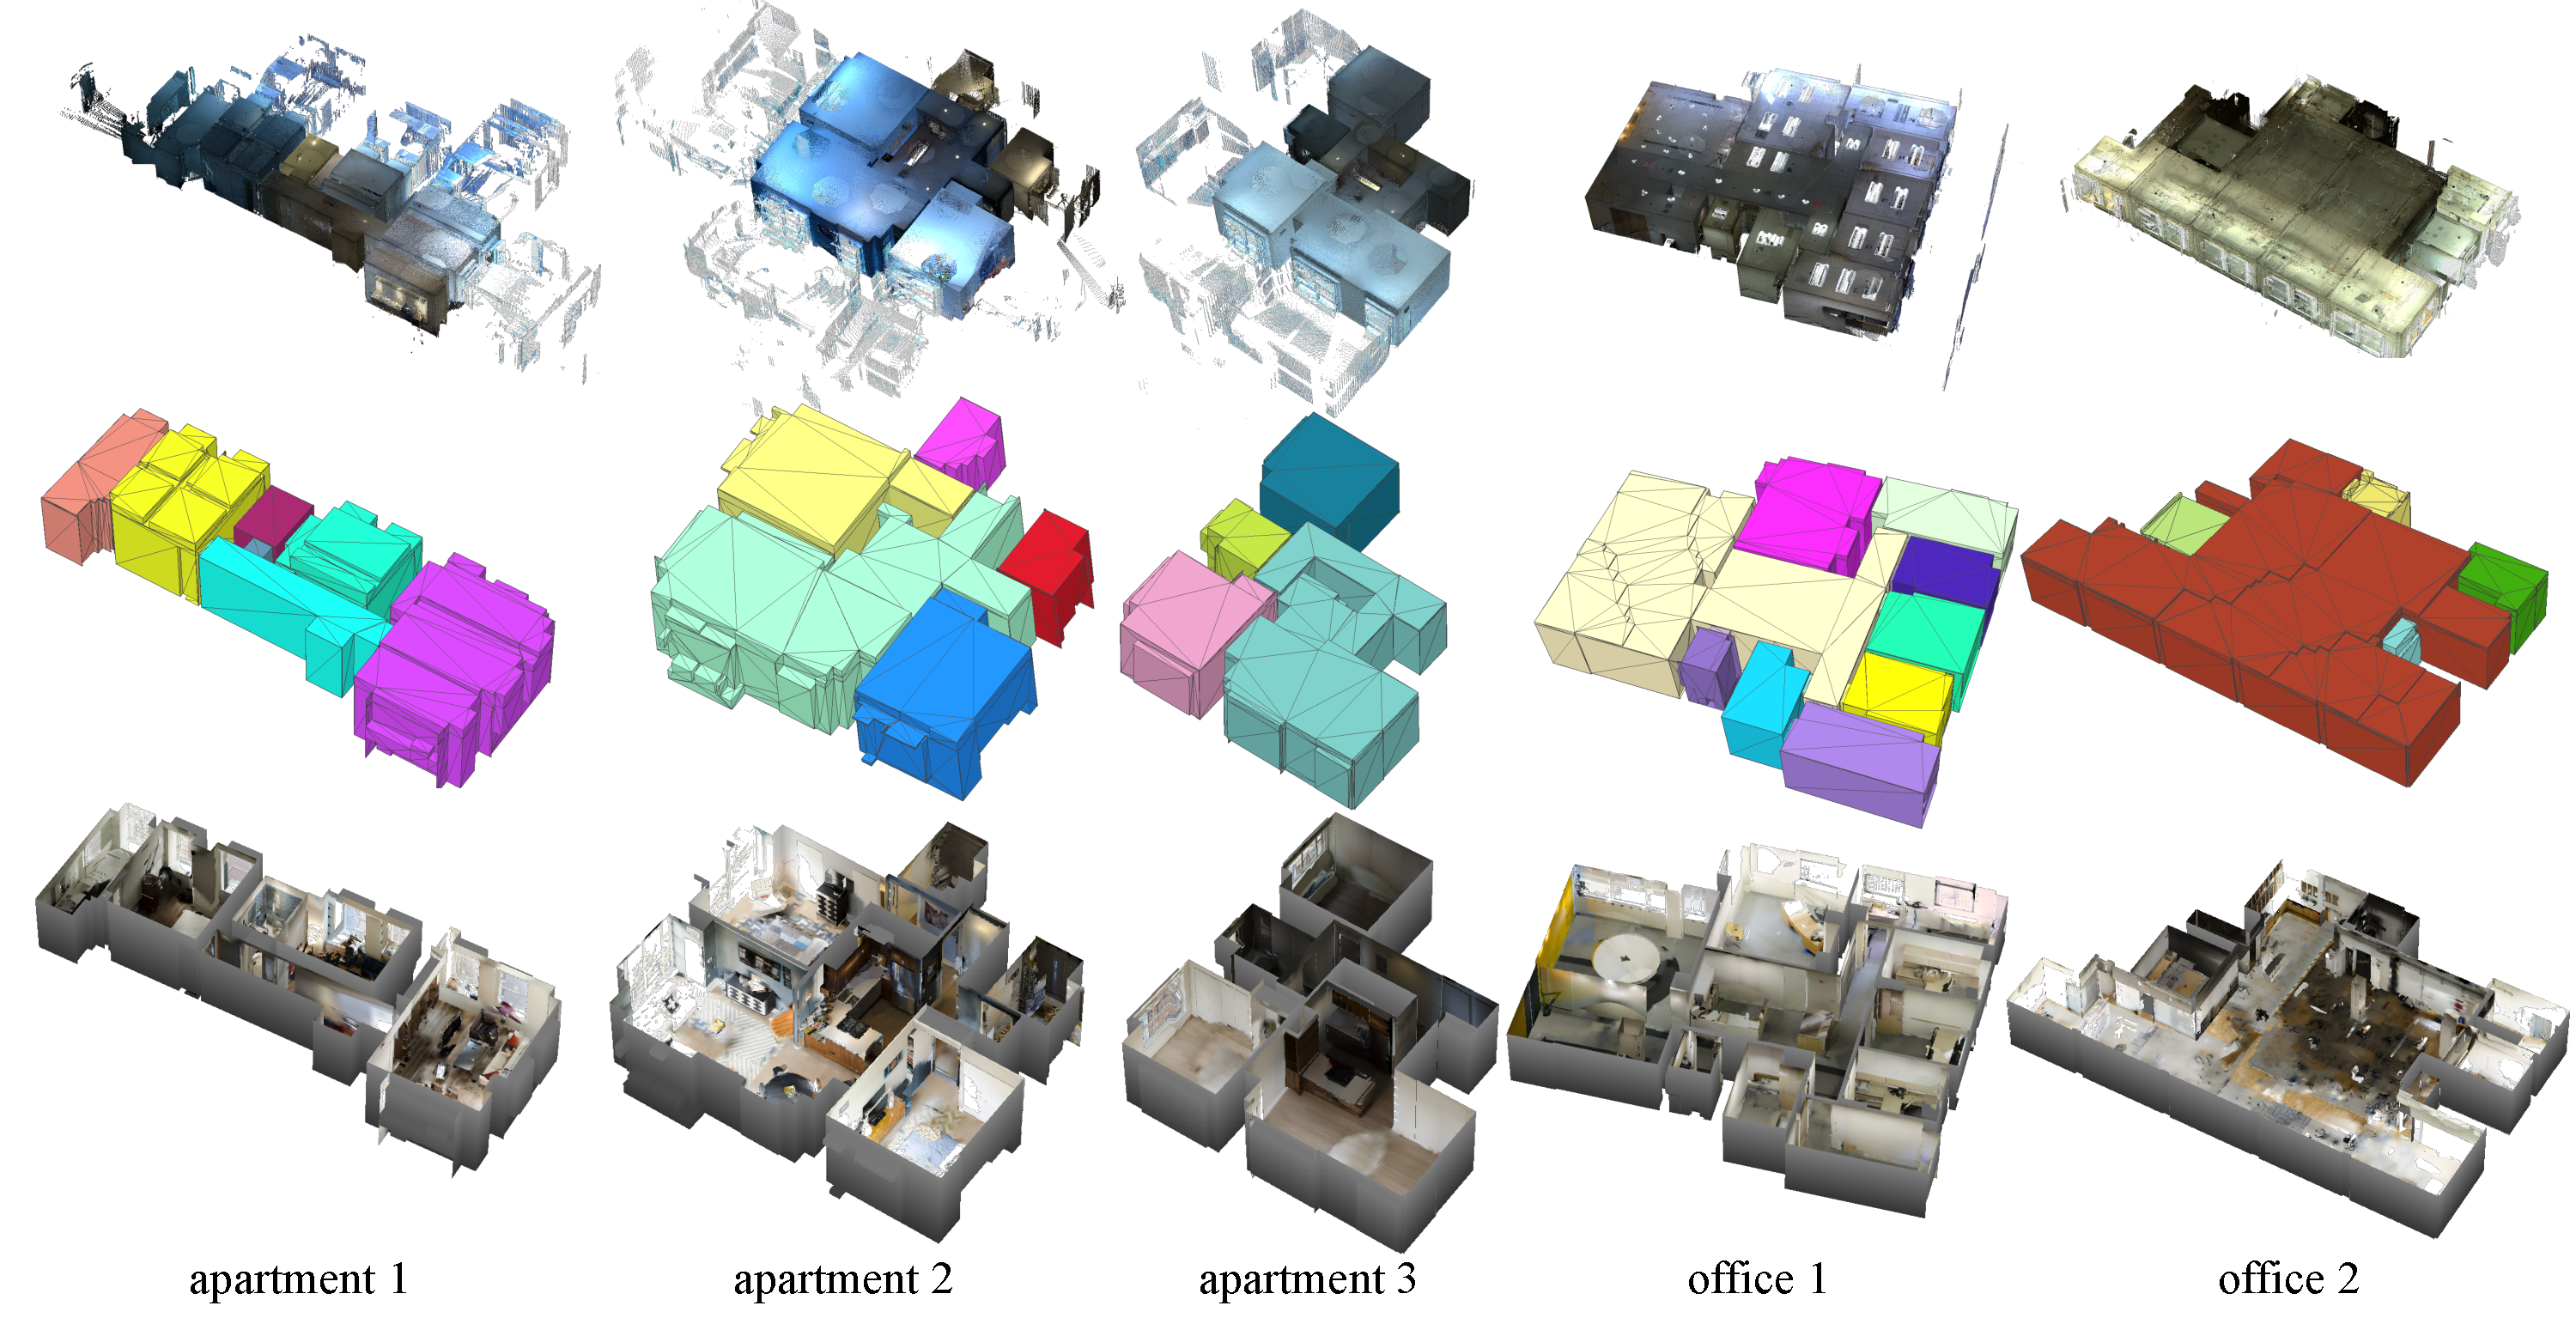
\includegraphics[width=150mm]{../figures/result_real.pdf}
\end{center}
 \vspace{-0.3cm}
\caption{Results on the real datasets.  From top to bottom: the input
 point clouds, the reconstructed mesh models, and sample renderings.}
 \label{fig:result_real}
 \vspace{-0.25cm}
\end{figure*}
\begin{table}[!t]
\caption{Statistics of the real experiments. Here we show the number of
 elements reconstructed and the geometric distance from the input depth
 map and reconstructed surface geometry compiled with (a) walls, (b)
 walls+details, (c) walls+details+objects. We also show the
 computational time of the entire pipeline.}
 \vspace{-0.5cm}
\begin{center}
\includegraphics[width=85mm]{../figures/statistics.pdf}
\end{center}
\label{table:statistics}
 \vspace{-0.7cm}
\end{table}
% We also evaluate our algorithm using five real datasets: a set of (1)
% {\it apartment } dataset (16 panoramas), (2) {\it apartment 2} dataset
% (15 panoramas), (3) {\it apartment 3} dataset (14 panoramas), (4) {\it
% office 1} dataset (33 panoramas), and (5) {\it office 2} dataset (35
% panoramas). \footnote{The number of points or examples of actual
% panorama images are shown in the supplementary.}
Unlike the synthetic datasets, 3D points in the real datasets are corrupted by
mirrors, windows, reflective objects, and calibration errors.
%
%
The second row in Fig.~\ref{fig:result_real} shows the reconstructed
meshes, compiled from the leaf nodes except for objects in the
structure graph. The color of each geometry is determined by the
parent room node. The third row shows the full renderings including the
object point clouds, which are rendered by the point-based rendering
technique. Note that ceiling geometries are not rendered on purpose to
visualize the interior, which is not easy for polygon soup mesh
models.
% More evaluations are provided in the supplementary material.
%
% At the second rows, we show the reconstructed manifold meshes compiled
% with room, wall, floor, ceiling, and their children details excluding
% the objects node (room segmentation is illustrated by color).
%At the third rows, the texture mapped models compiled with object nodes
%are illustrated. Since we do not have ground truth surfaces, it is quite
%hard to quantitatively evaluate these results, however
%We can qualitatively judge the quality of the results
%by examining the texture-mapped model at the third rows, since if the
%geometry is incorrect, it gives the unnatural sense when looking at the
%textured model.
%
%
%
Although it is difficult to conduct quantitative evaluations on real
datasets, Table~\ref{table:statistics} provides positional errors (the
same metric as in Table~\ref{table:quantitative}) of our model with and
without the wall details and the object point clouds.
More evaluations including qualitative and quantitative comparisons
against Poisson and Vgcuts meshes are provided in the supplementary material.


% Furthermore, we also give statistics
% of our reconstruction in each major steps. In addition, we give the
% total distance between the reconstructed geometry and input point clouds
% that explains how each configuration fits to the input. It is worth
% noting that while the reconstruction of the structured graph takes time,
% the compilation of the model is quite fast since the mesh/point cloud
% have already been attached to the element and we can immediately output
% the model if the leaf nodes are selected.



% \begin{figure}[!t]
% 	\begin{center}
% 		\includegraphics[width=85mm]{../figures/comp_segmentation.pdf}
% 	\end{center}
% 	\caption{\yasu{rotate and flip equal sky from zurich}Comparison of the room segmentation algorithms. Here we show the result of real dataset (a) lumber-cashew, (b) equal-sky, (c) red-lion, (d) new-breeze, and (e) salmon-palace. The first rows are the segmentation result by~\cite{Turner2015}, and the second rows are our room segmentation results. At the third rows, we also show the input point cloud where the points that are higher than camera positions are removed.}
% 	\label{fig:result_berkeley}
% \end{figure}


Figure~\ref{fig:comp_samemesh} qualitatively compares our
reconstructions against Poisson and Vgcuts. Again, the mesh
simplification algorithm~\cite{Tarini2010} and the parameter tuning is
used to make their polygon counts close to ours. The figure shows that
both Poisson and Vgcuts models contain clutters. Instead, our approach
successfully ignores clutters in modeling architectural components,
yielding clean building structure. These clean models enable high
quality texture mapping and rendering experiences, as well as,
interesting post geometry processing.
\begin{figure}[!t]
\begin{center}
\includegraphics[width=85mm]{../figures/comp_samemesh.pdf}
\end{center}
 \vspace{-0.3cm}
\caption{Comparison with the same number of triangular meshes. Here we show the result of (a)Poisson, (b) Vgcuts, and (c) ours. Note that we simplify the original meshes of Poisson and Vgcuts so that the models contain the same number of polygons with ours.}
\label{fig:comp_samemesh}
 \vspace{-0.25cm}
\end{figure}

We compare our room segmentation process against two state-of-the-art
methods~\cite{Mura2014,Turner2015} in Fig.~\ref{fig:result_all}.  We
asked the authors to process our data. Our method provides reasonable
segmentation that mostly preserves the number of structural cluster
(\eg, room, aisle) and important details.
%, although occasionally produce under-segmented results (\eg, office1).
The over-segmentation is often observed in~\cite{Turner2015}, and the
room shape is too simplified and important details often disappear
in~\cite{Mura2014}. Note that the results could not be obtained for
three datasets by ~\cite{Mura2014}, mainly due to the failures in the
primitive extraction step.
\begin{figure}[!t]
\begin{center}
\includegraphics[width=85mm]{../figures/result_all.pdf}
\end{center}
 \vspace{-0.2cm}
\caption{Comparison of the room segmentation algorithms. The first and
second rows are the results by~\cite{Mura2014} and
\cite{Turner2015}, respectively. The third rows contain ours. The bottom
 rows show the input point clouds for reference.}  \label{fig:result_all}
 \vspace{-0.25cm}
\end{figure}



% Finally, we show the experimental results that show our algorithm can
% easily control the complexity of the manifold meshes, which will be
% important for mobile application, where the rendering power varies
% depending on the device but is limited. In this experiment we control
% the complexity of the mesh by three parameters the maximum number of
% meshes about (entire scene, each room, each wall). Then our system
% automatically generate the manifold meshes by cutting off leaf nodes so
% that the constraint is satisfied. We show some examples of the meshes
% in~\Fref{fig:complexity2}.


% \begin{figure}[!t]
% \begin{center}
% \includegraphics[width=85mm]{../figures/shortestpath.pdf}
% \end{center}
% \caption{Comparison of the surface meshes of the real dataset. Here we show the result of (a) ours, (b) SCPoission, and (c) VGCuts. The same number of polygons are used for each model.}
% \label{fig:shortestpath}
% \end{figure}

%\begin{figure}[!t]
%\begin{center}
%\includegraphics[width=85mm]{../figures/complexity.pdf}
%\end{center}
%\caption{We can compile the manifold meshes from a structured graph by changing the deepest nodes to be compiled. Here we show three examples where (a) wall nodes, (b) wall and their children detail nodes, and (c) wall, detail, and object nodes are compiled.}
%\label{fig:shortestpath}
% \vspace{-0.25cm}
%\end{figure}


\section{Applications} \label{section:applications}
The structured scene representation facilitates novel applications.  In
this paper, we demonstrate the following four.
Please also see our supplementary video.

\mysubsubsection{Floorplan generation}
%Given the precise shape and segmentation of architectural components,
The first application is the generation of floorplan images. One missing
information is the types of objects and rooms, which are obtained by
state-of-the-art object recognition
software~\cite{berkeley_object_detection_software} and scene recognition
software~\cite{mit_scene_demo_paper}.
%Simply throwing the panorama images did not work well, in particular for
%the scene recognition, and we have experimented several different
%algorithms to generate input images.
% Due to the space limitation,
Experimental details and evaluations are in the supplementary material.
% We restrict our description to the most interesting finding here, while
% referring the rest to the supplementary material. The scene recognition
% did not work well with the panorama images, and we render $400\times
% 300$ standard perspective images with the horizontal field of view of
% $90$ degrees. The results depend on the viewing directions and we
% experimented with the four algorithms as shown in
% Table~\ref{table:scene}.  The first algorithm, for example, picks the
% panorama closest to the room center, renders six uniformly overlapping
% images, and picks the scene type with the best average score. This
% performs the worst. The best algorithm looks at all the panorama images
% that are inside the room, but uses the single rendered image in which
% the room is the most visible in the top-down view. An observation is
% that poorly positioned panoramas tend to yield incorrect results but
% with very high confidence. A rather better strategy is to use the best
% viewing direction from the best panorama.
In addition to placing annotation texts,
%on the floorplan image,
we can automatically change the rendering style of each room and object
depending on its type.
%(\eg, background color and texture) and/or each object (\eg, icon
%choices).
%Please see our supplementary video for examples.

\mysubsubsection{Indoor scene viewer} Our model enables a
novel indoor scene viewer, which renders an indoor scene from ground to
air, shows the floorplan image, displays room thumbnails,
or highlights room structures.
%or visualizes the relationships among different structural elements.
Room elements serve as interactive icons to enable a room-based
navigation.

\mysubsubsection{Inverse-CAD} The mesh model compiled from the structure
graph is compact, yet regularized, and a manifold. We can export our
model to a CAD system (\eg Sketchup~\cite{sketchup} as COLLADA format)
for users to easily fix mistakes, add new structures, or clone new rooms
within a minute or two.

\mysubsubsection{Tunable reconstruction} As mobile applications
dominate, it becomes crucial to intuitively and directly control the
complexity of a model, because the computational powers of mobile
devices vary but are limited.
%Existing methods typically offer only scalar weights inside an energy
%function to control model smoothness. They are far from intuitive and
%often not effectivein controlling the model complexity.
%provide almost no effective control over the model complexity,
The structure graph allows us to,
%intuitively control the complexity of an output model,
for example, specify the maximum number of poygons allowed for an entire
scene (X), each room (Y), and each wall (Z). We simply repeat dropping
leaf nodes until these constraints are all satisfied (See
Fig.~\ref{fig:complexity_control}).
\begin{figure}[!t]
\begin{center}
\includegraphics[width=85mm]{../figures/complexity2.pdf}
\end{center}
 \vspace{-0.2cm}
\caption{Structured model representation allows one to
 directly specify the
 % intuitively  control the complexity of an output manifold mesh, in particular, the
 maximum number of polygons allowed for an entire scene (X), each room
 (Y), and each wall (Z). The values of $(X,Y,Z)$ are $(2000,500,100)$,
 $(1000, 500, 2)$, and $(500, 100, 10)$ from left to right in the figure.
 When the budget is really tight (right), the
 system might drop a few rooms. %, yet the model is a manifold without gaps
 % or holes, and prevents artifacts in rendering and simulation.
 %
%  Mesh complexity control based on our graph structure. Using our
% model representation, we can easTily control the complexity of manifold
% meshes for each element-level. In this example, we fix the maximum
% number of meshes about (entire scene, each room, each wall) and then
% automatically compiled corresponding meshes. The mesh models at (left)
% is more complex than (middle), and some room geometry was dropped in
% (right) but the manifold-ness is still satisfied. \yasu{this will be
%  important for mobile application, where the rendering power varies
%  depending on the device but  is limited. The manifold mesh without gaps
%  and holes is ideal for rendering and simulation.
 }
\label{fig:complexity_control}
 \vspace{-0.25cm}
\end{figure}

% Note that most existing reconstruction algorithms usually provide a few
% mysterious parameters (\eg, scalar weights in the MRF formulation),
% where these parameters are non-intuitive, and resultant models are
% highly unpredictable.

%         %algorithm and exact parameters. Can you provide here?} We also
% %remove objects that are near walls, which can be represented by room
% mesh model \yasu{again how exactly?}. To do this, we discretize the 3D
% room space to $64\times 64\times 64$ voxels and mark voxels that are
% occupied by room structures as 1 and all others as 0. After dialating
% the voxel grid, we remove objects whose more than 75\% of points are
% inside voxels with value 1. The next step is to re-assign colors to
% objects points from panoramas since the original colors are not
% reliable. The key point here is to select a minimum set of panoramas
% from which the most points of the object can be clearly seen. Given an
% object, we initialize all points as unseen, and greedily search for
% panoramas in which the object occupies largest area in image domain, and
% most unseen points become seen. To compensate for exposure difference
% between panoramas, we also estimate a $3\times 3$ color transform matrix
% between two panoramas using the points that can be seen from both of
% them.

\section{Limitations and Future Directions}

This paper presents a novel structured model representation and
reconstruction algorithm.
%, which is driven by the structure grammar defining the structural
%relationships of scene elements.
We admit that our current system has limitations. First, the most
problematic step is the connection classification. Our current approach
relies only on local geometric information, and tends to under-segment.
% Our classification rule is fairly complex and a future work is to
A future work is to exploit images to robustify the classification
process. Scene and object recognition accuracies are also poor at many
places, where building-scale context from the structure graph may
help. For example, a bedroom is unlikely to be in the middle of offices.
%structured scene representation at the scale of an entire building, much
%bigger than a single image and a panorama.
%structural regularities and patterns are persistent abundant in the same building.
%Our structured model representation provides much bigger context in a
%building scale, which has a potential to further boost the
%performance.
%%For example, in the same building,
%chairs and tables tend to have the same shape, and
%%windows tend to have the same shape and be at the same height.
%(for object detection).
% It is unlikely to see a bedroom in the middle of conference
%rooms (for scene recognition).
Another future work is to test our framework on RGBD stream datasets as
opposed to panorama RGBD images. Although the camera pose quality tends
to degrade for RGBD streams, our framework should be applicable.
% We have chosen to work on the latter for several reasons. First, the
% camera pose quality tends to degrade for RGBD streams, especially for
% challenging scenes.  Second, the panorama experience is becoming an
% industry standard for scene visualization~\cite{google-maps,matterport},
% which is not easy to achieve from RGBD streams.
% %the lack of an ability to turn around exposes significant drawbacks in
% %real applications.

We hope that
%The datasets and the source code will be shared with the research
%community.
this paper opens up a number of new exciting research directions such as
the following. Please visit our project website~\cite{SIMProject} for
more information, source code, and datasets.
%, and share the source code and the datasets at the project
% and facilitates novel industrial applications.

\mysubsubsubsection{Structured X modeling} Structured modeling is a
general framework, and is applicable to many other domains such as
outdoor architectural scenes or man-made objects.
%outdoor scenes or man-made objects.
%Structured modeling framework should be applicable outside the
%indoor scenes. Structured outdoor modeling or structured object modeling
%is an interesting space to also explore.
%

\mysubsubsubsection{Indoor Inverse Procedural Modeling} Structure
grammar is manually constructed in our experiments. An interesting
alternative is to learn the grammar rules from examples.

\mysubsubsubsection{Inverse-CAD and Scan2BIM} Inverse-CAD has been a
long-standing research milestone in Computer Vision, Computer Graphics,
and Civil Engineering.  For major architectural components, our models
already enable practical human post-processing. This research could
serve as a good stepping stone to tackle an even harder Scan2BIM
problem.

\yasu{a bit strange finish}

\section*{Acknowledgment}
This research is supported by National Science Foundation under grant IIS 1540012. We thank Floored Inc. for providing us with the dataset and support. We thank Eric Turner and Claudio Mura for running their code on our datasets for evaluation.
\clearpage
{\small
	\bibliographystyle{ieee}
	\bibliography{egbib,furukawa}
}

	
\end{document}
